%% This is file `elsarticle-template-1-num.tex',
%%
%% Copyright 2009 Elsevier Ltd
%%
%% This file is part of the 'Elsarticle Bundle'.
%% ---------------------------------------------
%%
%% It may be distributed under the conditions of the LaTeX Project Public
%% License, either version 1.2 of this license or (at your option) any
%% later version.  The latest version of this license is in
%%    http://www.latex-project.org/lppl.txt
%% and version 1.2 or later is part of all distributions of LaTeX
%% version 1999/12/01 or later.
%%
%% The list of all files belonging to the 'Elsarticle Bundle' is
%% given in the file `manifest.txt'.
%%
%% Template article for Elsevier's document class `elsarticle'
%% with numbered style bibliographic references
%%
%% $Id: elsarticle-template-1-num.tex 149 2009-10-08 05:01:15Z rishi $
%% $URL: http://lenova.river-valley.com/svn/elsbst/trunk/elsarticle-template-1-num.tex $
%%
\documentclass[preprint,12pt]{elsarticle}

%% Use the option review to obtain double line spacing
%% \documentclass[preprint,review,12pt]{elsarticle}

%% Use the options 1p,twocolumn; 3p; 3p,twocolumn; 5p; or 5p,twocolumn
%% for a journal layout:
%% \documentclass[final,1p,times]{elsarticle}
%% \documentclass[final,1p,times,twocolumn]{elsarticle}
%% \documentclass[final,3p,times]{elsarticle}
%% \documentclass[final,3p,times,twocolumn]{elsarticle}
%% \documentclass[final,5p,times]{elsarticle}
%% \documentclass[final,5p,times,twocolumn]{elsarticle}

%% if you use PostScript figures in your article
%% use the graphics package for simple commands
%% \usepackage{graphics}
%% or use the graphicx package for more complicated commands
%% \usepackage{graphicx}
%% or use the epsfig package if you prefer to use the old commands
%% \usepackage{epsfig}

%% The amssymb package provides various useful mathematical symbols
\usepackage{amssymb}
%% The amsthm package provides extended theorem environments
%% \usepackage{amsthm}

%% The lineno packages adds line numbers. Start line numbering with
%% \begin{linenumbers}, end it with \end{linenumbers}. Or switch it on
%% for the whole article with \linenumbers after \end{frontmatter}.
\usepackage{lineno}

%% natbib.sty is loaded by default. However, natbib options can be
%% provided with \biboptions{...} command. Following options are
%% valid:

%%   round  -  round parentheses are used (default)
%%   square -  square brackets are used   [option]
%%   curly  -  curly braces are used      {option}
%%   angle  -  angle brackets are used    <option>
%%   semicolon  -  multiple citations separated by semi-colon
%%   colon  - same as semicolon, an earlier confusion
%%   comma  -  separated by comma
%%   numbers-  selects numerical citations
%%   super  -  numerical citations as superscripts
%%   sort   -  sorts multiple citations according to order in ref. list
%%   sort&compress   -  like sort, but also compresses numerical citations
%%   compress - compresses without sorting
%%
%% \biboptions{comma,round}

% \biboptions{}

\usepackage{subfigure}
\usepackage{fancyvrb}

\newcommand{\A}{$\alpha$}
\newcommand{\CA}{$\alpha$-carbon}
\newcommand{\SAP}{{\tt SAP}}
\newcommand{\DALI}{{\tt DALI}}
\newcommand{\Tab}[1]{Table~\ref{Tab:#1}}
\newcommand{\Fig}[1]{Figure~\ref{Fig:#1}}
\newcommand{\Eqn}[1]{Equ$^n$.~\ref{Eqn:#1}}

\journal{Structure}

\begin{document}

\begin{frontmatter}

%% Title, authors and addresses

%% use the tnoteref command within \title for footnotes;
%% use the tnotetext command for the associated footnote;
%% use the fnref command within \author or \address for footnotes;
%% use the fntext command for the associated footnote;
%% use the corref command within \author for corresponding author footnotes;
%% use the cortext command for the associated footnote;
%% use the ead command for the email address,
%% and the form \ead[url] for the home page:
%%
%% \title{Title\tnoteref{label1}}
%% \tnotetext[label1]{}
%% \author{Name\corref{cor1}\fnref{label2}}
%% \ead{email address}
%% \ead[url]{home page}
%% \fntext[label2]{}
%% \cortext[cor1]{}
%% \address{Address\fnref{label3}}
%% \fntext[label3]{}

\title{A comparative analysis of the foamy and ortho virus capsid structures
           reveals an ancient domain duplication}

%% use optional labels to link authors explicitly to addresses:
\author[label1]{William~R.~Taylor}
\author[label2]{Jonathan~P.~Stoye}
\author[label3]{Ian~A.~Taylor}
\address[label1]{Computational Cell and Molecular Biology,}
\address[label2]{Retrovirus-Host Interactions,}
\address[label3]{Macromolecular Structure Laboratory.}
\address{Francis Crick Institute, 1 Midland Rd., London NW1 1AT, UK}


\begin{abstract}
%% Text of abstract
The {\em Spumaretrovirinae} (foamy viruses) and the {\em Orthoretrovirinae} (e.g. HIV) share
many similarities both in genome structure and the sequences of the core viral encoded proteins,
such as the aspartyl protease and reverse transcriptase.  Similarity in the Gag region of the 
genome is less obvious at the sequence level but has been illuminated by the recent solution of
the foamy virus capsid (CA) structure.   This revealed a clear structural similarity to the 
orthoretrovirus capsids but with marked differences that left uncertainty in the relationship
between the two domains that comprise the structure.   Using multiple structure comparison
methods combined with statistical tests, we have shown that the relationship of the two domains
conforms to a simple linear correspondence rather than a domain transposition.   These
similarities suggest that the origin of both viral capsids was a common ancestor with a double
domain structure.  In addition, we show that there is also a significant structural similarity 
between the amino and carboxy domains in both the foamy and ortho viruses which suggests that
there may have been an even more ancient gene-duplication that preceded the double domain structure.
\end{abstract}

\begin{keyword}
Virus capsid structure \sep foamy virus evolution \sep protein structure comparison
%% keywords here, in the form: keyword \sep keyword

%% MSC codes here, in the form: \MSC code \sep code
%% or \MSC[2008] code \sep code (2000 is the default)

\end{keyword}

\end{frontmatter}

%%
%% Start line numbering here if you want
%%
\linenumbers

%% main text
\section{Introduction}

Taxonomically, the {\em Orthoretrovirinae} (orthoretroviruses) and {\em Spumaretrovirinae}\footnote{
This class is also commonly referred to as the Foamy viruses (after the morphological effect they have on infected cells)
and will be referred by this name frequently below, with the term orthoretroviruses also contracted to "Ortho viruses".
}
(spumaviruses) make up the two subfamilies of {\em Retroviridae}. They share many similarities, including overall genome
structures with gag, pol and env genes encoding proteins for replication and life cycles involving reverse transcription
and integration into the chromosomes of infected cells. However, there are also a number of differences distinguishing these
viral subfamilies, including finer details of genome organisation, the absence of a Gag-Pol fusion protein in spumaviruses
and the timing of reverse transcription \cite{LindemannDet11}.

Gag is the major structural protein of both Ortho and Foamy viruses and is responsible for many of the differences and
similarities between the viral subfamilies. Ortho and Foamy viral Gags are required for particle assembly, budding from the
cell, reverse transcription and delivery of the viral nucleic acid into the newly infected cell. However, there are a number
of striking differences including how the Gag precursor is targeted to the cell membrane, the absence of a Major Homology
Region and Cys-His box in Foamy viruses and very different patterns of processing during viral maturation \cite{MullersEet13}. 
In all Ortho viruses, Gag is proteolytically cleaved to form distinct, well-studied proteins, matrix (MA), capsid (CA) and 
nucleocapsid (NC), found in mature virions, whilst in spumaviruses Gag processing to remove a C-terminal peptide occurs 
only in a fraction of the Gag molecules \cite{FlugelRMet03}. 

Structural information regarding foamy virus Gag has been limited to the crystal structure of the N-terminal Env binding
region of Prototypic Foamy virus (PFV) Gag (PFV-Gag-NtD) that although maintaining some of the function of orthoretrivial
MA shared no structural similarity \cite{GoldstoneDCet13}. However, more recently the solution NMR structure of the PFV Gag 
central CA domains has shed new light on the relationship between ortho and spumaviruses. It reveals that the CA structures 
of both viral subfamilies share a common protein fold, implying that their Gag proteins may be evolutionarily related 
\cite{BallNJet16}. 

However, an intriguing aspect of this relationship was an ambiguity in the degree of relatedness between the CA domains 
of the Gag proteins, with the Spumaretroviral CA domains, NtDCEN and CtDCEN, appearing almost equally similar to either 
the amino- (CA-NtD) or carboxy-terminal (CA-CtD) domains of the orthoretroviruses. In this paper, we now investigate and 
clarify the nature of this relationship and discuss its evolutionary implications.


\section{Results}

\subsection{Full-length comparison}

To investigate the structural relationship between the capsid structure of the ortho viruses (HIV, MLV, etc.),
and the new structure of the foamy virus capsid \cite{BallNJet16} (PDB codes: 5m1g, 5m1h), the foamy virus structure was
compared to one of the few full double domain ortho virus structures, the HIV capsid with PDB code: {\tt 3nte},
using the flexible superposition program \SAP\ \cite{TaylorWR99a}.   Even though this program has a tolerant approach
to relative domain shifts, the comparison produced a high RMSD value of 14\AA\ over the 100 best superposed
positions.   The amino (N) terminal domain positions roughly corresponded but shifts in the relative
orientation of the carboxy (C) terminal domain resulted in large deviations between equivalent helices.
The superposed structures are shown in \Fig{fullSAP} and the domain divergence can be seen clearly as a
jump in the cumulative RMSD plot (\Fig{fullRMS}).

\begin{figure}
\centering
\subfigure[]{
\label{Fig:fullSAP}
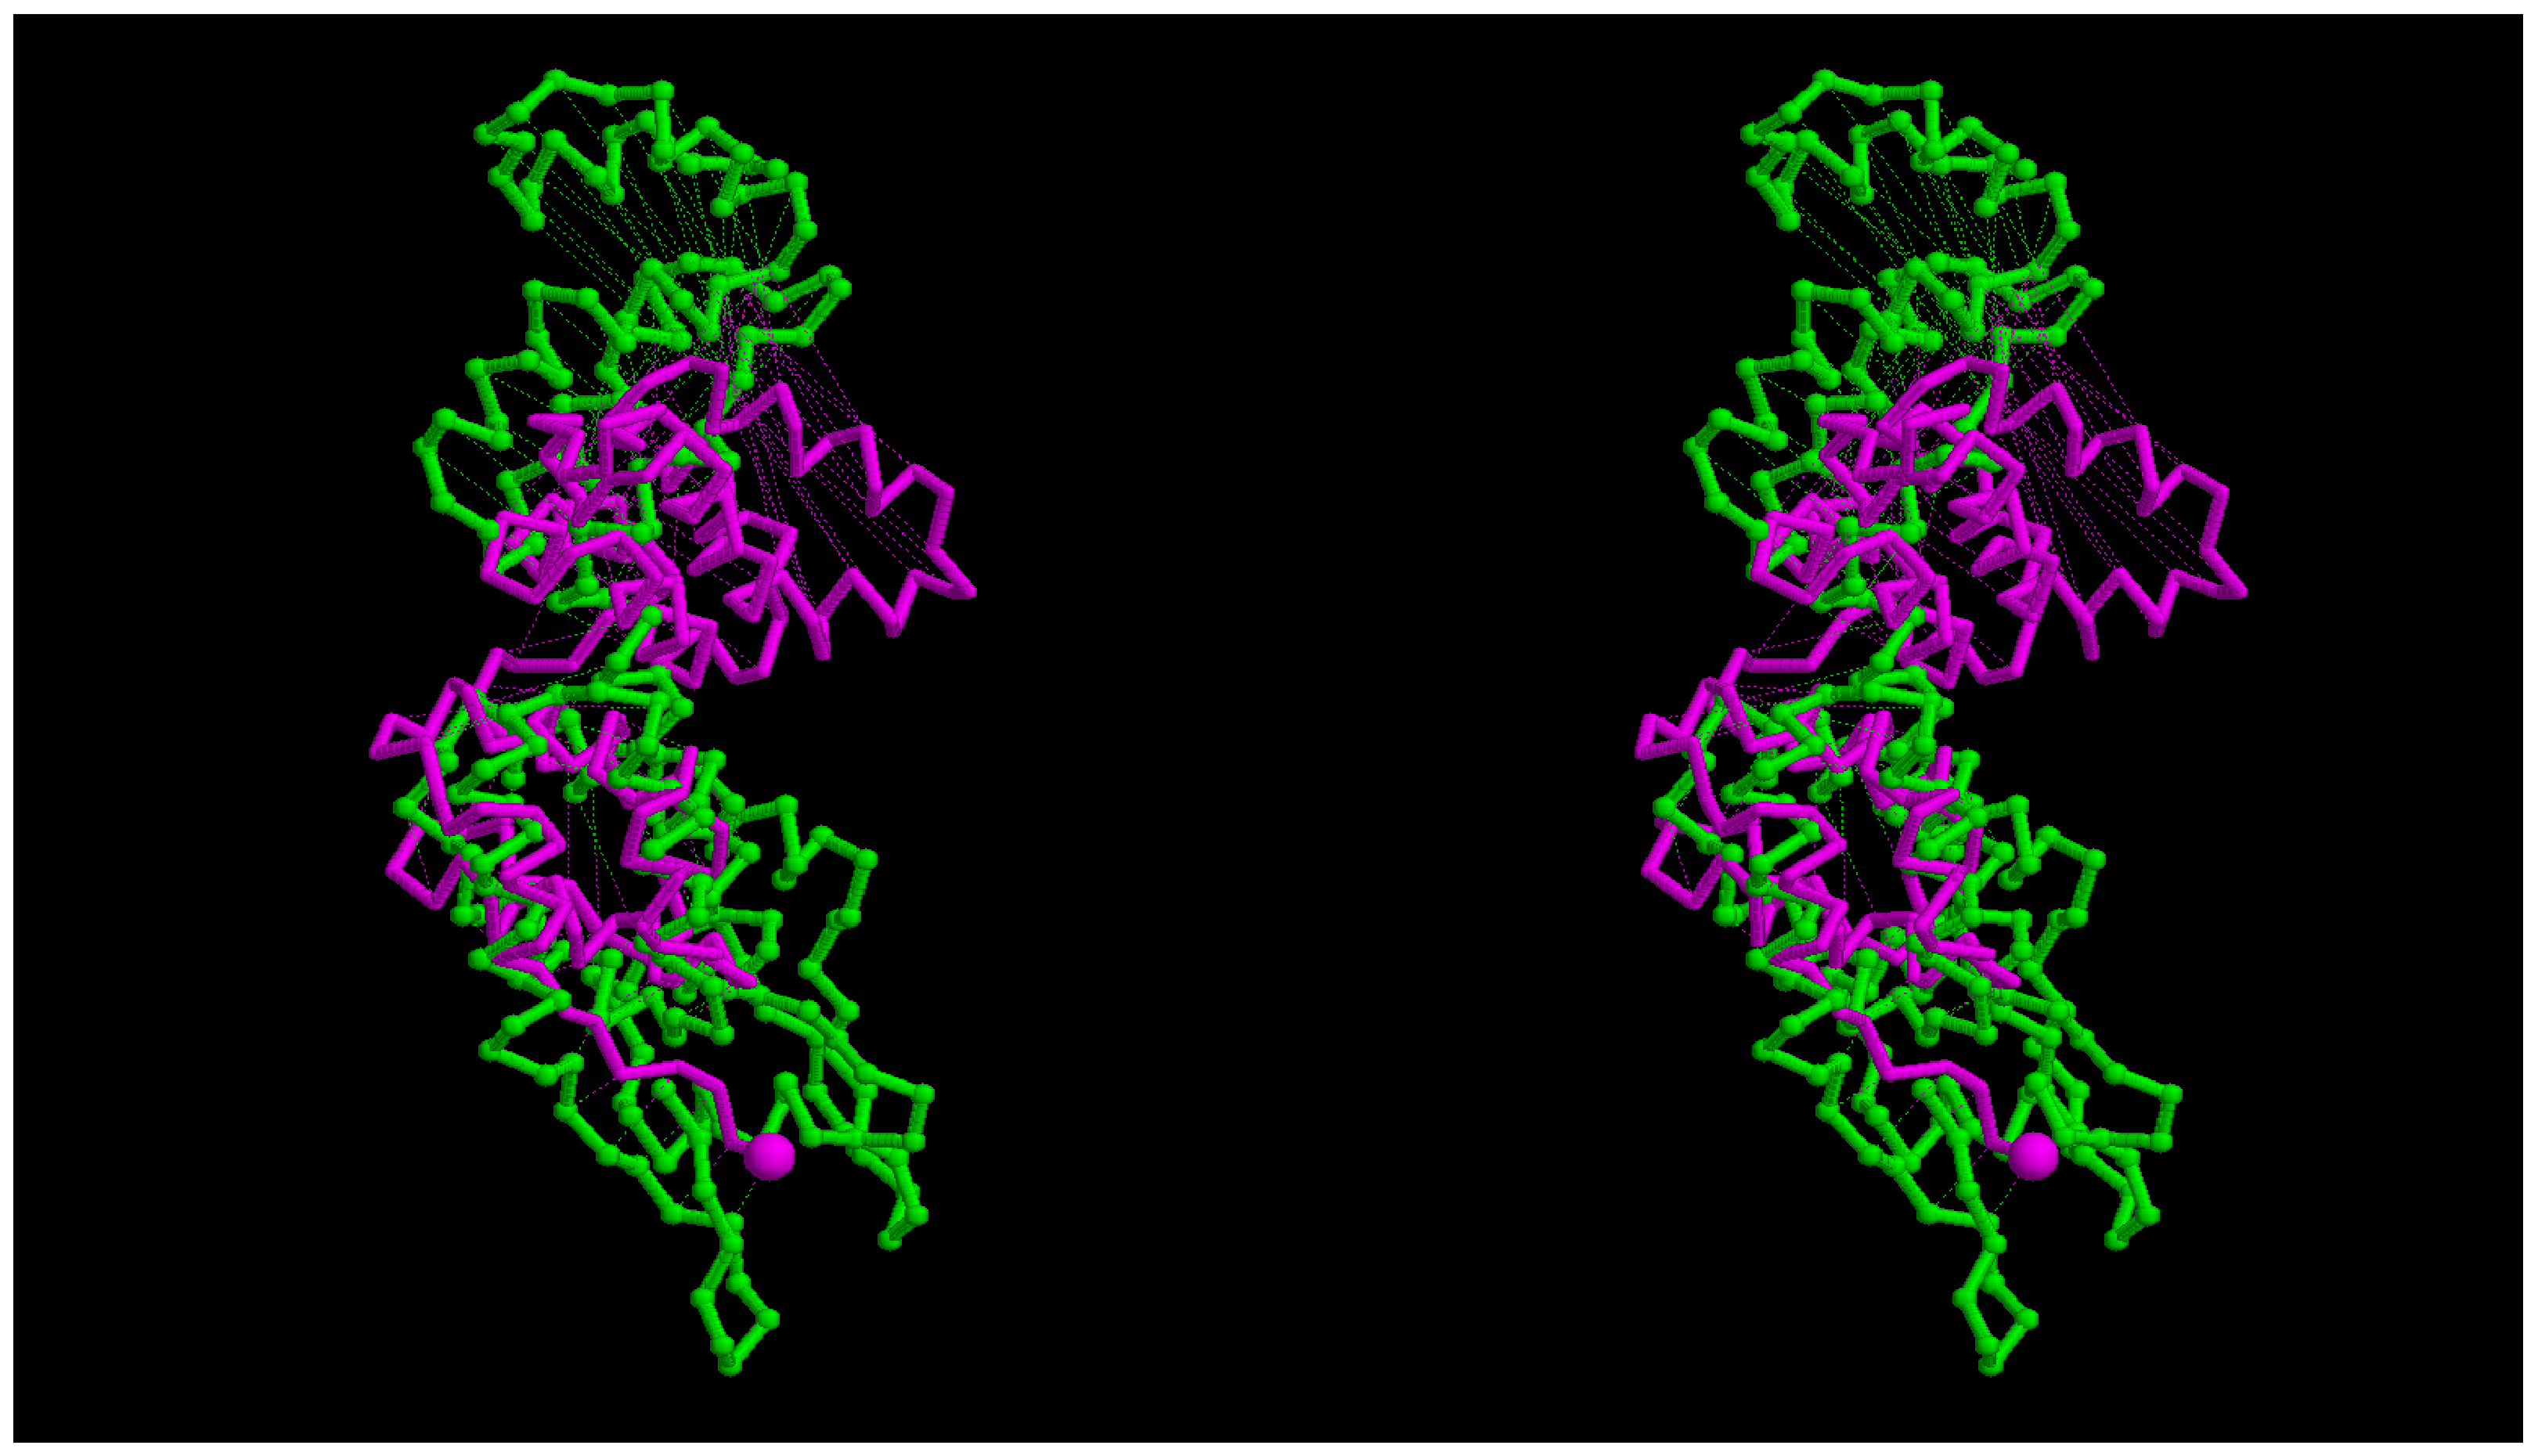
\includegraphics[width=300pt]{full3nte-super.eps}
}
\subfigure[]{
\label{Fig:fullRMS}
\rotatebox{270}{
\includegraphics[width=220pt]{plotrms.eps}
}}
\begin{footnotesize}
\caption{
\label{Fig:full}
{\bf Full ortho/foamy virus capsid superposition}.
The superposed structures are shown in part ($a$) as a stereo pair, coloured as green = ortho virus (HIV, PDB code: {\tt 3nte-A})
and magenta = foamy virus capsid.   (The amino terminus is marked by a small sphere).
Part ($b$) shows the cumulative RMSD plot for this superposition which plots the RMSD value (Y-axis) for increasingly larger sets
of residues as ranked by their \SAP\ similarity score (X-axis).   The sharp rise in this trace marks the transition into
subsets that include positions from the displaced domain.
}
\end{footnotesize}
\end{figure}

\subsection{DALI searches}

Although this initial superposition (\Fig{full}) did not appear encouraging, the foamy virus structure
was scanned across the Protein DataBank (PDB), using the \DALI\ program \cite{HolmLet93a} to search for any similarities.

\subsubsection{Full chain scan}

A scan of the full-length foamy structure using the DALI server\footnote{
{\tt http://ekhidna.biocenter.helsinki.fi/dali\_server},
see Methods section for details.
}
over the 90\% non-redundant protein structure databank
identified a wide selection of retroviral capsid structures.  In the ranked list of structure hits,
capsids were identified from position 2 to position 550.
The top hits are shown in \Fig{dali} (See Supplementary material for a summary of
the full 550 with Z-scores over 2).    Many capsids are found in the top 20 hits and although the top
scoring hit is not obviously a capsid protein, it is thought to have originated from the Ty3/Gypsy
retrotransposon family gag gene \cite{ZhangWet15}.   However, almost all of these are partial
hits, covering little more than half the query structure.   The structural alignment of the top two hits
is shown in \Fig{top2} coloured to emphasise the matched regions.

\begin{figure}
\centering
\begin{tiny}
\begin{Verbatim}[frame=single]
   No:  Chain   Z    rmsd lali nres  %id PDB  Description
    1:  4x3x-A  5.0  3.1   66    82   11 PDB  MOLECULE: ACTIVITY-REGULATED CYTOSKELETON-ASSOC
    2|  3g29-A  3.7  2.7   60    77    8 PDB  MOLECULE: GAG POLYPROTEIN;                                           
    3|  3g0v-A  3.7  2.9   62    76    8 PDB  MOLECULE: GAG POLYPROTEIN;                                           
    4:  2v50-D  3.6  2.2   41   998    7 PDB  MOLECULE: MULTIDRUG RESISTANCE PROTEIN MEXB;                         
    5:  3j39-i  3.6  2.5   40   113    3 PDB  MOLECULE: 60S RIBOSOMAL PROTEIN L10A-2;                              
    6|  4ph2-A  3.6  3.2   69   127    7 PDB  MOLECULE: BLV CAPSID - N-TERMINAL DOMAIN;                            
    7:  1iqp-E  3.6  3.8   69   326    7 PDB  MOLECULE: RFCS;                                                      
    8:  4gco-A  3.6  3.7   55   120   11 PDB  MOLECULE: PROTEIN STI-1;                                             
    9|  3g29-B  3.6  2.8   62    77    8 PDB  MOLECULE: GAG POLYPROTEIN;                                           
   10|  3g1i-B  3.6  2.9   62    75    8 PDB  MOLECULE: GAG POLYPROTEIN;                                           
   11|  3g21-A  3.6  2.8   60    77    8 PDB  MOLECULE: GAG POLYPROTEIN;                                           
   12:  2a0u-A  3.5  3.1   68   374    4 PDB  MOLECULE: INITIATION FACTOR 2B;                                      
   13:  1j7q-A  3.5  2.9   60    86    5 PDB  MOLECULE: CALCIUM VECTOR PROTEIN;                                    
   14:  2a0u-B  3.5  8.1   80   367    4 PDB  MOLECULE: INITIATION FACTOR 2B;                                      
   15:  1iqp-A  3.5  3.7   70   326    7 PDB  MOLECULE: RFCS;                                                      
   16|  4ph0-C  3.5  4.6  101   199    8 PDB  MOLECULE: BLV CAPSID;                                                
   17|  4ph0-D  3.5  4.2  101   198    8 PDB  MOLECULE: BLV CAPSID;                                                
   18|  4ph2-B  3.5  3.3   69   127    7 PDB  MOLECULE: BLV CAPSID - N-TERMINAL DOMAIN;                            
   19:  1sxj-B  3.4  3.5   65   316    3 PDB  MOLECULE: ACTIVATOR 1 95 KDA SUBUNIT;                                
   20:  2afd-A  3.4  2.7   59    88   14 PDB  MOLECULE: PROTEIN ASL1650;                                           
\end{Verbatim}
\end{tiny}
\begin{footnotesize}
\caption{
\label{Fig:dali}
{\bf Top structural similarities}
found by the \DALI\ program in the 90\% non-redundant PDB (PDB-90) using the full length foamy
virus capsid as a query (145 residues).
The columns are: the ranked number of the hit ({\tt No.}), marked by a '{\tt |}' for a capsid protein, otherwise '{\tt :}';
the PDB entry identifier ({\tt Chain}, with the chain designation after the dash); the \DALI\ Z-score ({\tt Z})
(significance estimate); the root-mean-square-deviation ({\tt rmsd}) over aligned \CA\ positions; the number
of aligned positions ({\tt lali}); the number of residues in the matched structure ({\tt nres}); the percentage
sequence identity of the match ({\tt \%id}) followed by a description of the molecule.
It can be seen from the number of matched positions ({\tt lali}) that most matches are partial,
covering typically less than half the query structure.
}
\end{footnotesize}
\end{figure}

\begin{figure}
\centering
\subfigure[{\tt 4x3x-A}]{
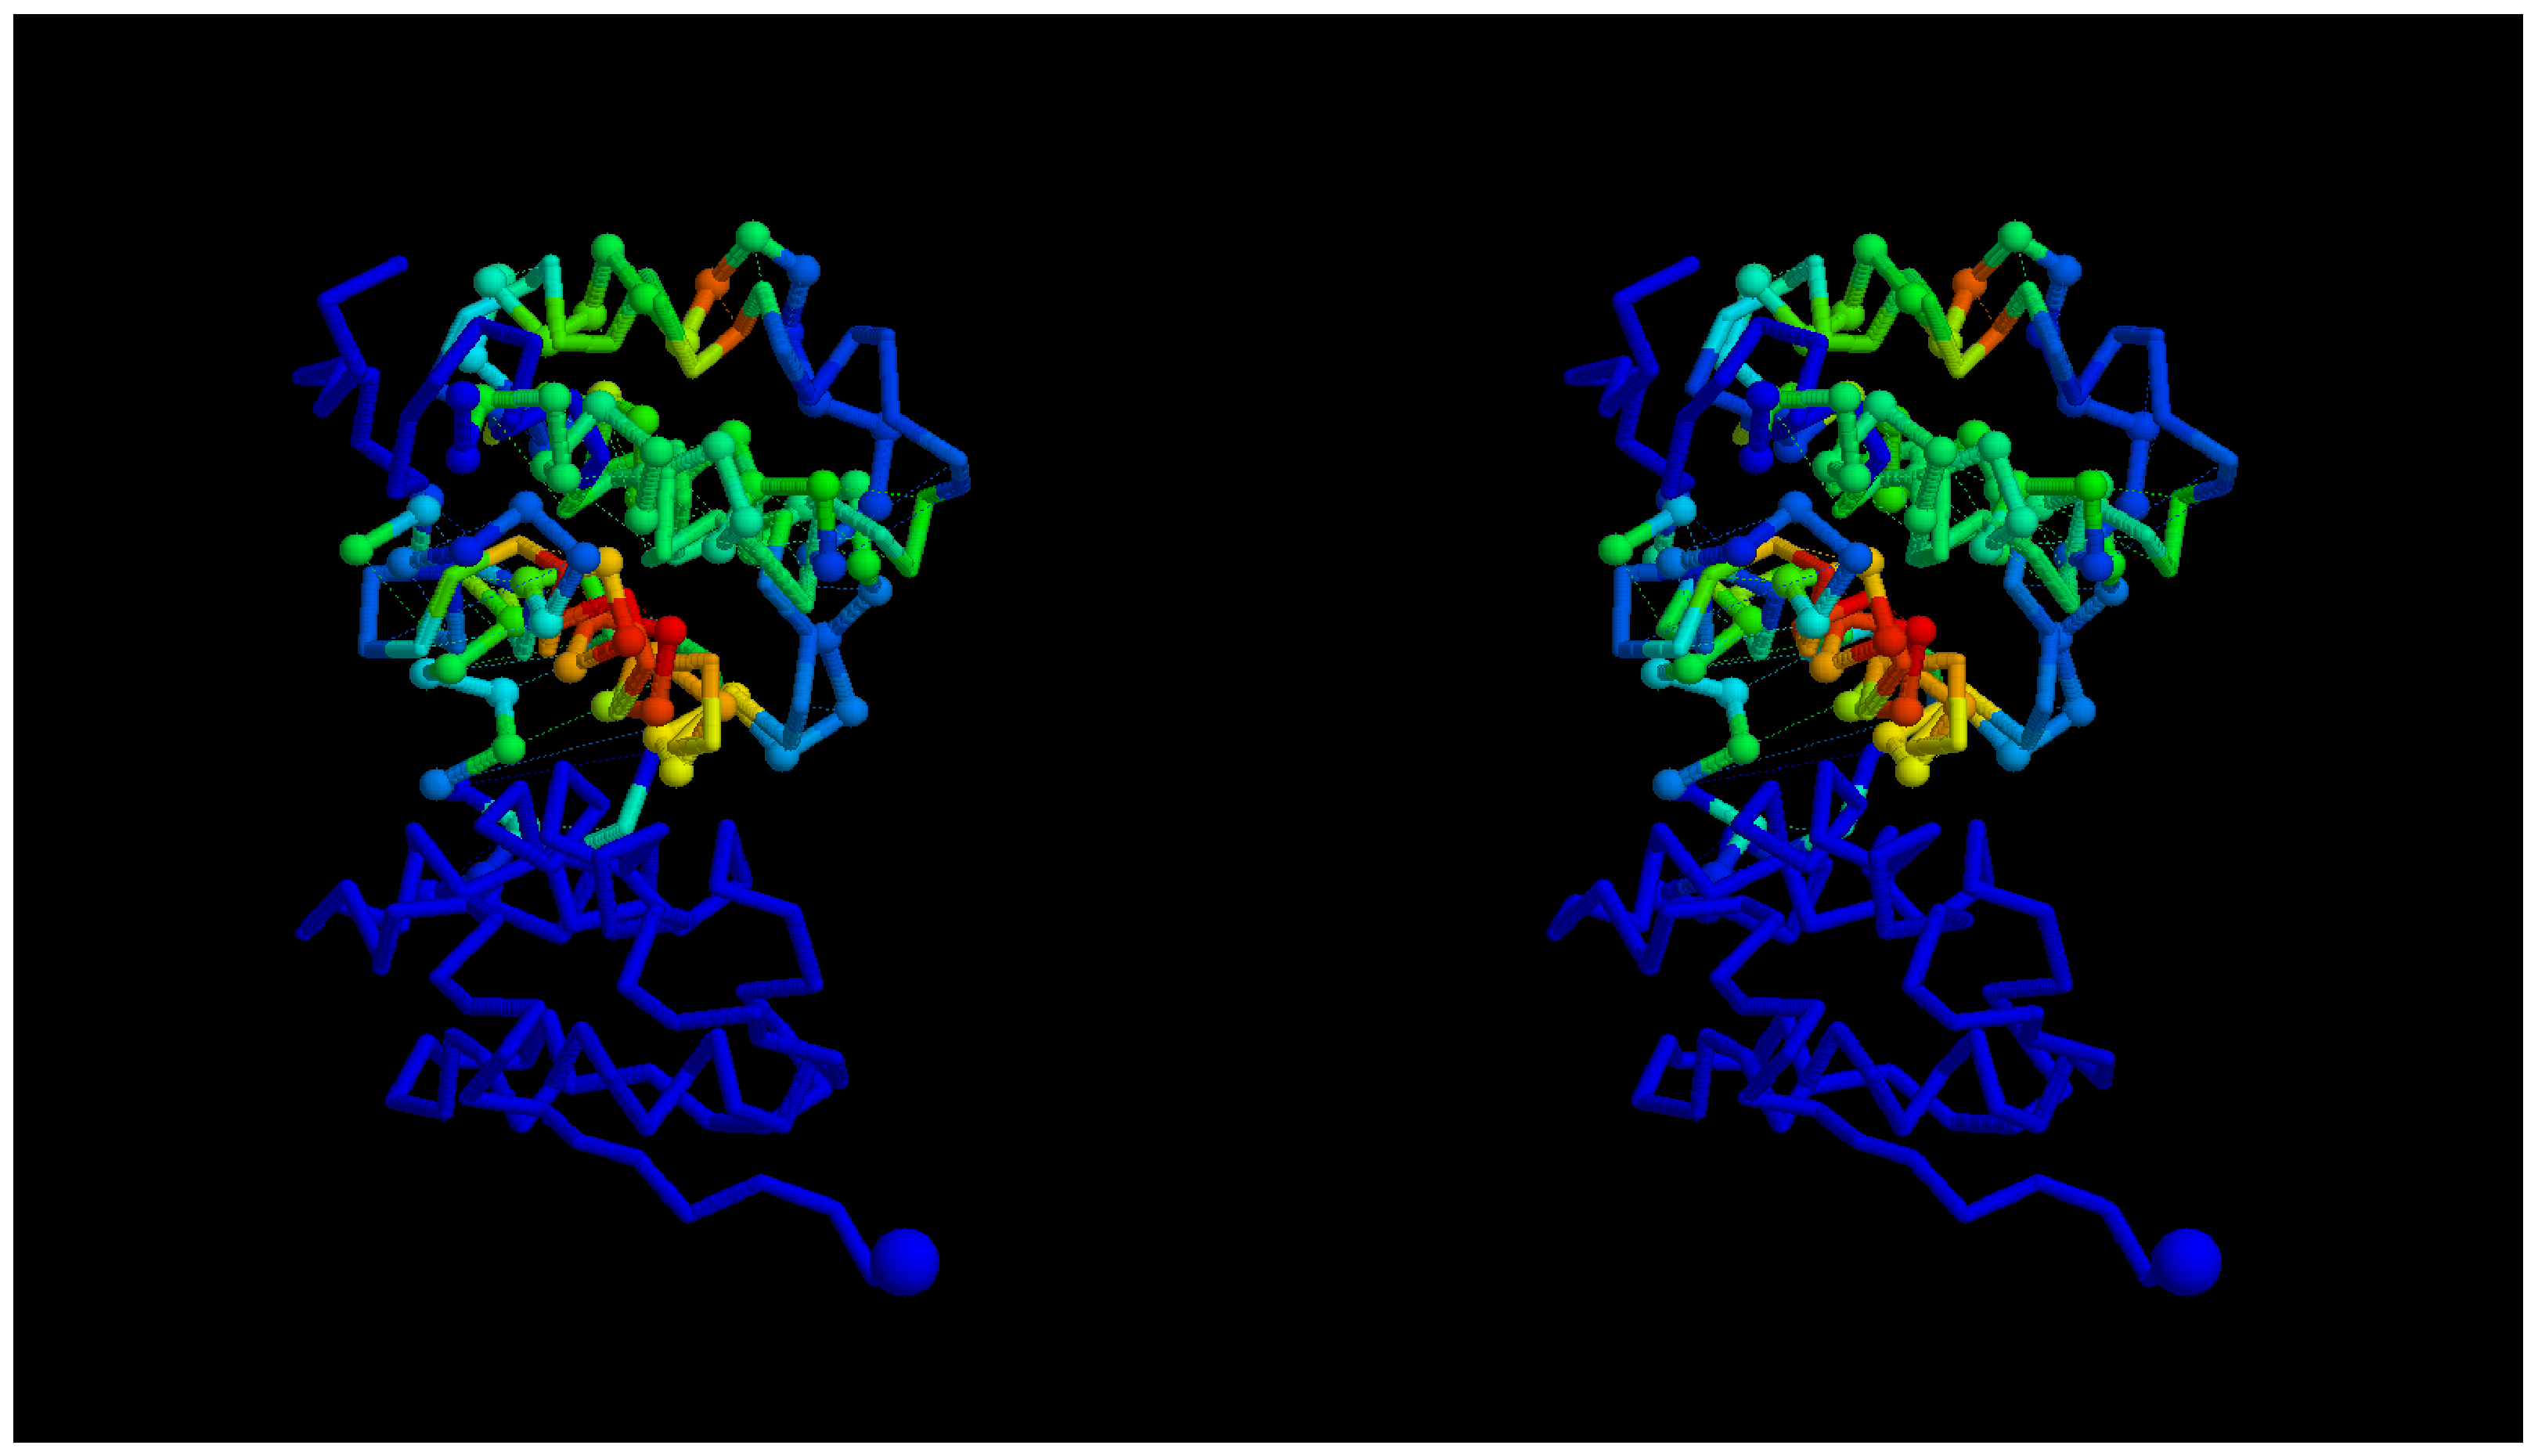
\includegraphics[width=300pt]{full4x3x-super.eps}
}
\subfigure[{\tt 3g29-A}]{
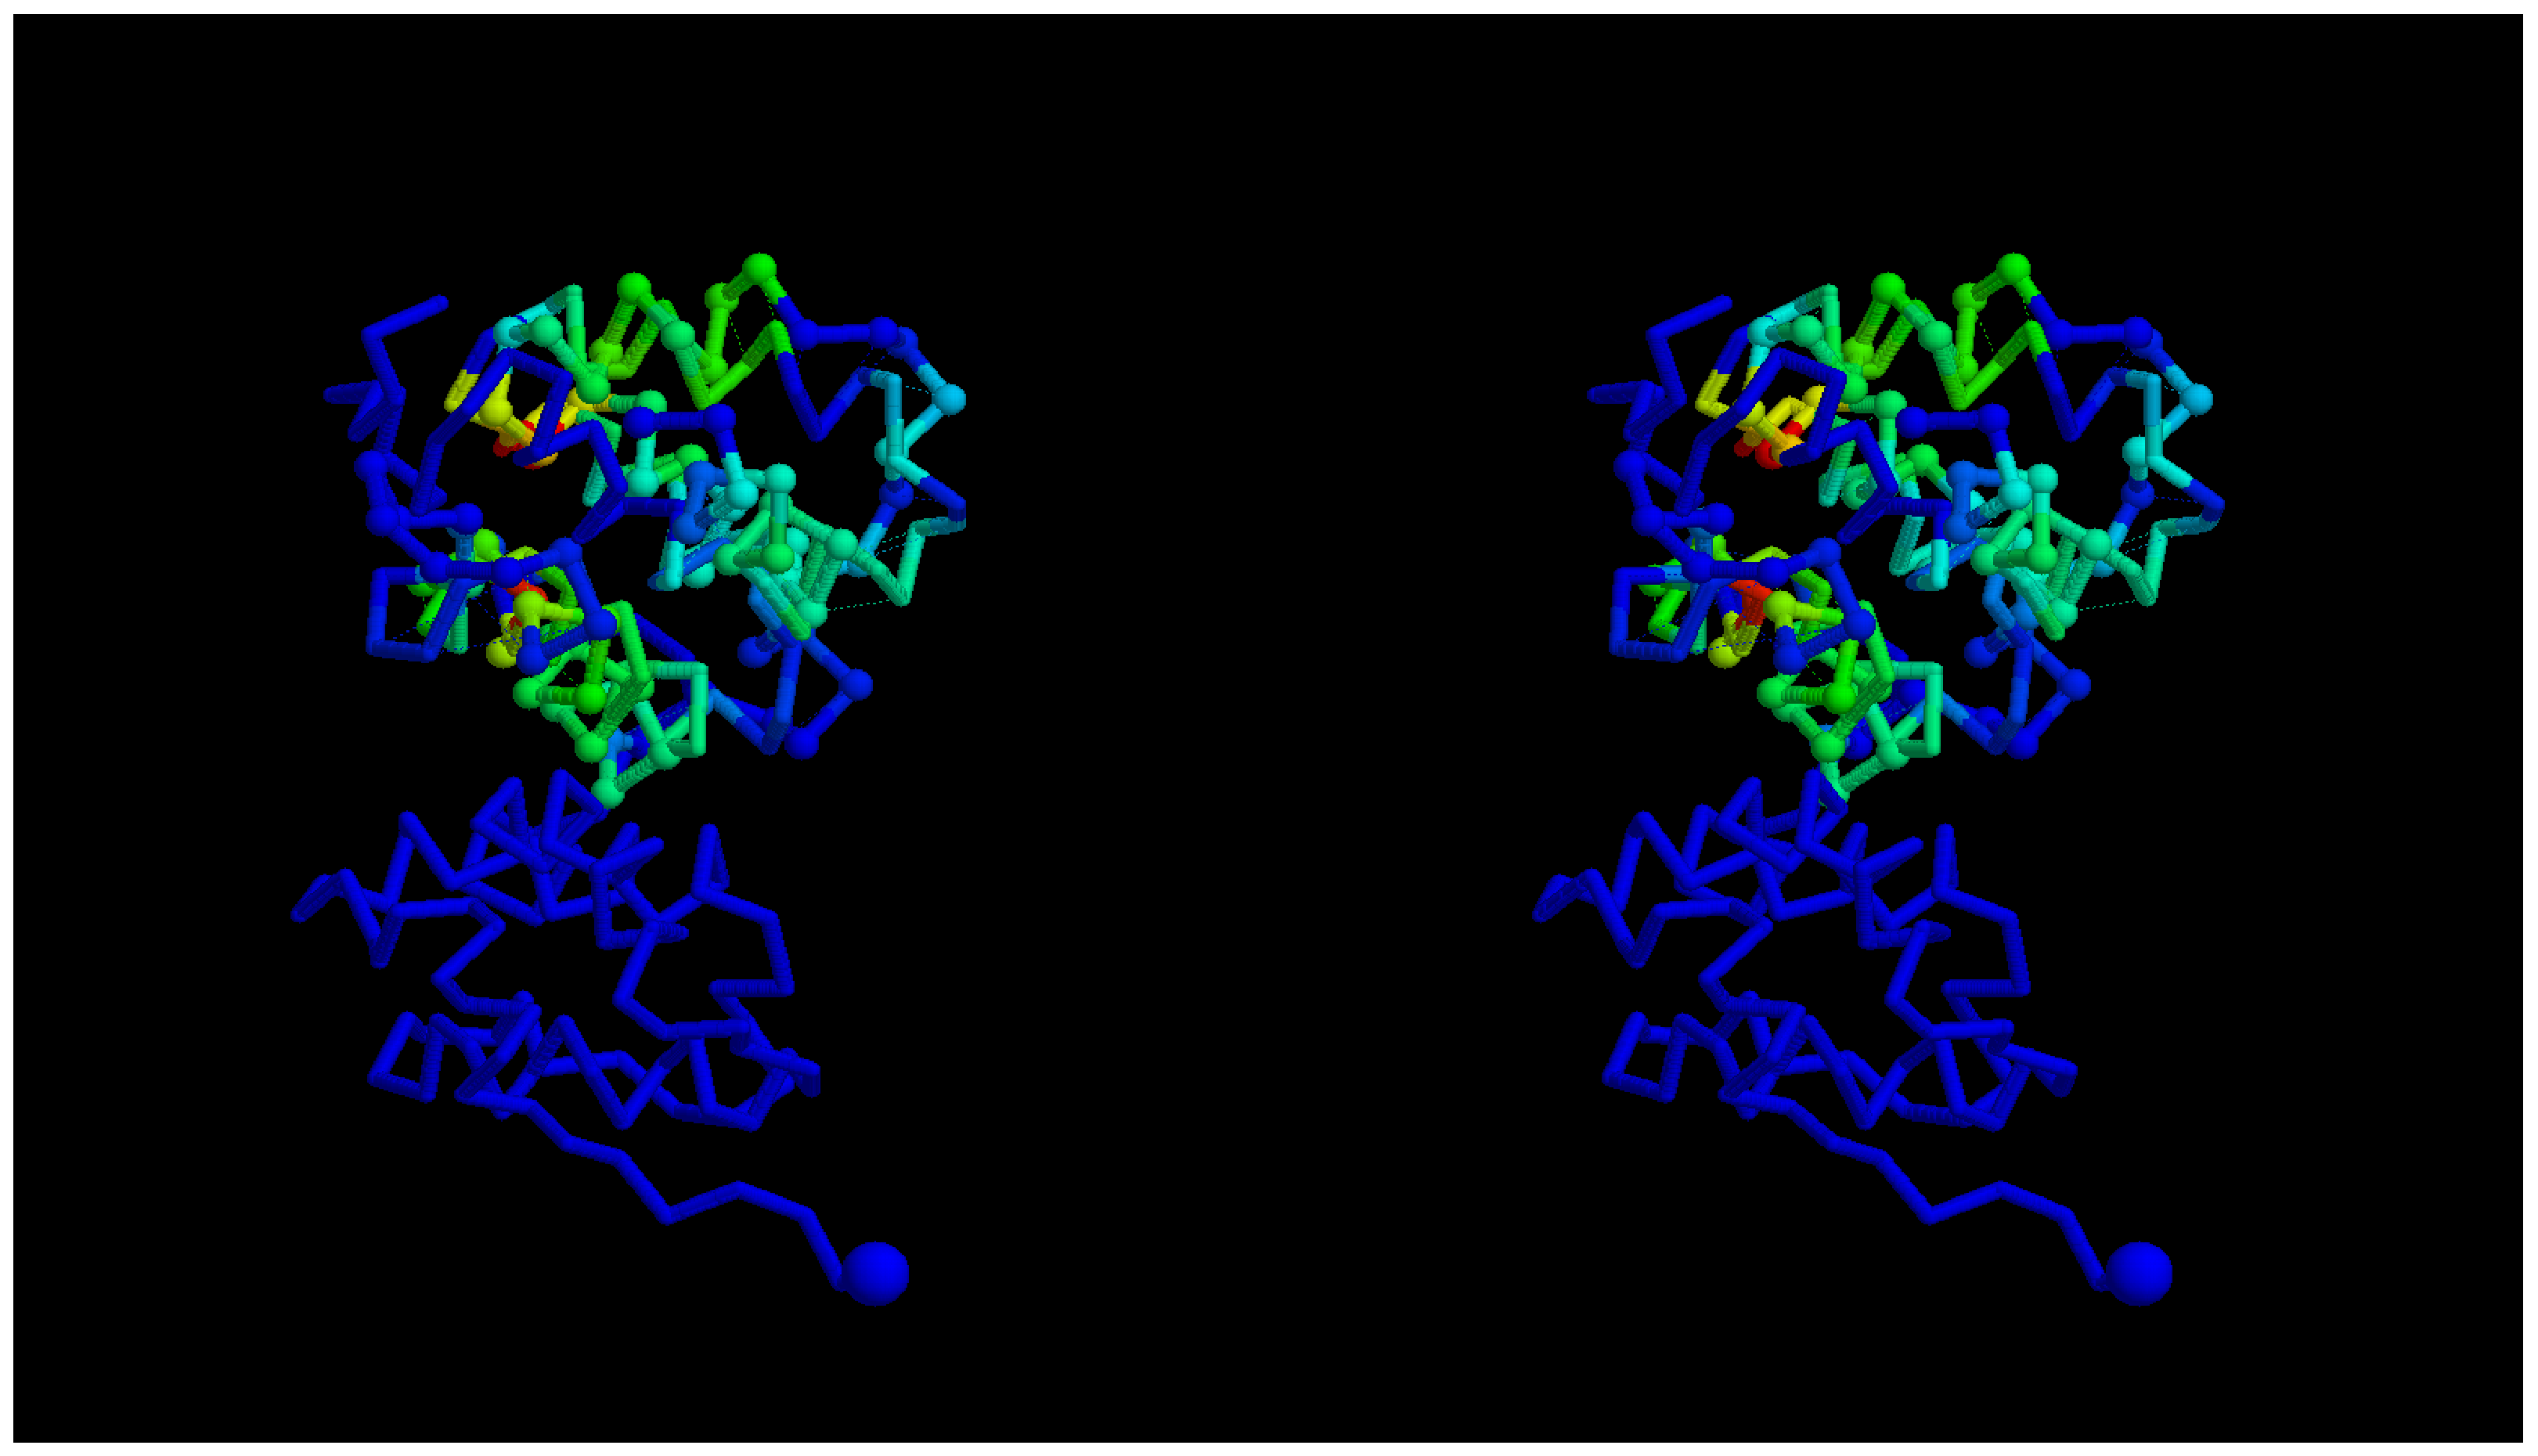
\includegraphics[width=300pt]{full3g29-super.eps}
}
\begin{footnotesize}
\caption{
\label{Fig:top2}
{\bf Top hits superposed}.
The top two \DALI\ hits to the full foamy virus capsid are shown as a \CA\ backbone (stereo pair) coloured using
the residue similarity score calculated by \SAP. (red = strong similarity, blue = none).
The amino terminus of the foamy structure is marked by a large ball and the other structure is distinguished
by small balls on its \CA\ atoms.
($a$) a cytoskeleton associated protein (fragment) of the arc/arg3.1 gene (PDB code: {\tt 4x3x-A}),
(which is thought to have originated from a Ty3/Gypsy retrotransposon family capsid)
and
($b$) the structure of the capsid C-terminal domain of the Rous scarcoma virus (PDB code: {\tt 3g29-A}).
}
\end{footnotesize}
\end{figure}

The result of the DALI search indicated that the Foamy virus structure shares some similarity with the
capsid structure of the ortho-viruses.  However, the matches consist only of a small number of
helices and appears barely more convincing than other matches to proteins that seem very unlikely
to have any meaningful connection to a viral capsid.   The preponderance of capsid matches
throughout the list of hits might seem to add some support to the relationship but may simply be
a reflection of the number of capsid structures in the structure databank.

Adding confusion to the ortho/foamy relationship is the additional observation that
the distribution of matches to the ortho-virus structures between the amino (N) and carboxy
(C) terminal domains are mixed.   For example; taking the top 10 matches, the N-terminal domain of the Foamy
structure aligns with 6 C-terminal domains and 4 N-terminal domains of the ortho virsuses
and the best match with the corresponding Foamy C-terminal domain aligns with an ortho N-terminal domain.

\begin{figure}
\centering
\subfigure[Full PDB]{
\label{Fig:daliFULL}
\rotatebox{270}{
\includegraphics[width=130pt]{dali-daliFULL-DALIhitROC.eps}
}}
\subfigure[PDB-90]{
\label{Fig:daliNR90}
\rotatebox{270}{
\includegraphics[width=130pt]{dali-daliNR90-DALIhitROC.eps}
}}
\begin{footnotesize}
\caption{
\label{Fig:rocs}
{\bf PDB capsid structure matches}.
The number of capsid structures identified by the \DALI\ program in ($a$) the full PDB and ($b$)
the 90\% non-redundant PDB (PDB-90) is shown for queries using the full foamy capsid
structure (red), the carboxy terminal domain (green) and the amino terminal domain (blue).
The number of capsid hits (Y-axis) is plotted against the order of all hits ranked by Z-score
down to a value of 2.   A curve approaching the top left corner indicates greater specificity
and the extent of a curve to the right indicates the total number of hits.
}
\end{footnotesize}
\end{figure}

\subsubsection{Domain scans}

To clarify the domain match specificity, the two domains of the Foamy virus (1--88 and 89--180,
as defined automatically \cite{TaylorWR99b}) were scanned separately using the \DALI\ program.
The individual domains were much more specific at matching known capsid structures\footnote{
True/false hits were defined by protein descriptions with the words "CAPSID", "GAG" or "P24".
},
both in the full PDB and PDB-90 collections as can be seen from the plots in \Fig{rocs}.

The results of these scans strengthened the identification
of the relationship to the ortho capsids and supported the swapped specificity for the N-terminal
match of the Foamy structure with the C-terminal match of the ortho virus and {\em vica versa}, with all
top 12 hits of each domain matching their opposed counterpart.
The structure-based sequence alignments of each domain based on this equivalence are shown in \Fig{swap}.

\begin{figure}
\centering
\begin{tiny}
\begin{Verbatim}[frame=single]
Nter    PIGTVIPIQHIRSVTGEPPRNPREIPIWLGRNAPAIDGVFPVTTPDLRCRIINAILGGNIGLSLTPGDCLTWDSAVATLFIRTHGTFP
                                :  :: |   |::|        :    ::        :        |    :  :: |      
3g1gA   ---------PWAD--IMQGPS--SFVDFANRLIKAVEGSDL-ARAPVIIDCFRQKSQPQQLI--PSTL-TTPGEIIKYVLDRQK----
3tirA   ---------PWAD--IMQGPS--SFVDFANRLIKAVEGSDL-ARAPVIIDCFRQKSQPQQLI-------TTPGEIIKYVLDRQ-----
3g1iA   ---------PWAD--IMQGPS--SFVDFANRLIKAVEGSDL-ARAPVIIDCFRQKSQPQQLI----TLTT-PGEIIKYVLDRQ-----
3g29A   ---------PWAD--IMQGPS--SFVDFANRLIKAVEGS---ARAPVIIDCFRQKSQPQQLI-------TTPGEIIKYVLDRQ-----
3g0vA   ---------PWAD--IMQGPS--SFVDFANRLIKAVEGSAL-ARAPVIIDCFRQKSQPQQLI-------TTPGEIIKYVLDRQ-----
3g29B   ---------PWAD--IMQGPS--SFVDFANRLIKAVEGSNL-ARAPVIIDCFRQKSQPQQLI-------TTPGEIIKYVLDRQ-----
3g1iB   ---------PWAD--IMQGPS--SFVDFANRLIKAVEGSDL-ARAPVIIDCFRQKSQPQQLI-------TTPGEIIKYVLDRQ-----
3g26A   ---------PWAD--IMQGPS--SFVDFANRLIKAVEGS---CRAPVIIDCFRQKSQPQQLI-------TTPGEIIKYVLDRQ-----
3dtjC   ---------SILD--IRQGPK--EPFRDYVDRFYKTLR--VKNW--MTATLLVQNANPD-TILKGPGA--TLEEMMTA-CQGV-----
3dtjB   ---------SILD--IRQGPK--EPFRDYVDRFYKTLR--VKNW--MTATLLVQNANPD-TILKGPGA--TLEEMMTA-CQGV-----
3dtjA   ---------SILD--IRQGPK--EPFRDYVDRFYKTLR--VKNW--MTATLLVQNANPD-TILKGPGA--TLEEMMTA-CQGV-----
3g21A   ---------PWAD--IMQGPS--SFVDFANRLIKAVEGSDL-ARAPVIIDCFRQKSQPQQLI-------TTPGEIIKYVLDRQ-----

Cter    MHQLGNVIKGIVDQEGVATAYTLGMMLSGQNYQLVSGIIRGYLPGQAVVTALQQRLDQEIDNQTRAETFIQHLNAVYEILGLNARGQSIRL
             |:   :|::   : ::::     |     :  :::     ||:: :|:: :::|:  :     :|  || :  :    
1l6nA   SPRTLNAWVKVVEEKA-IPMFSALSE---GATPDLNTMLNTVGGHQAAMQMLKETINEEA--EIYKRWIILGLNKIVRMYS------PTSI
3j34U   SPRTLNAWVKVVEEKA-IPMFSALSE--GATPQDLNTMLNTVGGHQAAMQMLKETINEEA--EIYKRWIILGLNKIVRMY-------SPTS
4u0bF   SPRTLNAWVKVVEEKA-IPMFSALSC--GATPQDLNTMLNTVGGHQAAMQMLKETINEEA--EIYKRWIILGLNKIVRMY-------SPTS
4u0bG   SPRTLNAWVKVVEEK--IPMFSALSC--GATPQDLNTMLNTVGGHQAAMQMLKETINEEA--EIYKRWIILGLNKIVRMY-------SPTS
3h4eB   SPRTLNAWVKVVEEK--IPMFSALSC--GATPQDLNTMLNTVGGHQAAMQMLKETINEEA--EIYKRWIILGLNKIVRMY-------SPTS
2jprA   SPRTLNAWVKVVEEKA-IPMFSALSE--GATPQDLNTMLNTVGGHQAAMQMLKETINEEA--EIYKRWIILGLNKIVRMY-----------
1afvB   SPRTLNAWVKVVEEKAVIPMFSALSE--GATPQDLNTMLNTVGGHQAAMQMLKETINEEA--EIYKRWIILGLNKIVRMY-------SPTS
4u0bE   SPRTLNAWVKVVEEK--IPMFSALSC--GATPQDLNTMLNTV-GHQAAMQMLKETINEEA--EIYKRWIILGLNKIVRMY-------SPTS
4u0bK   SPRTLNAWVKVVEEK--IPMFSALSC--GATPQDLNTMLNTVGGHQAAMQMLKETINEEA--EIYKRWIILGLNKIVRMY-------SPTS
4u0bH   SPRTLNAWVKVVEEK--IPMFSALSC--GATPQDLNTMLNTVGGHQAAMQMLKETINEEA--EIYKRWIILGLNKIVRMY-------SPTS
2gonA   SPRTLNAWVKVVEEK-VIPXFSALSE--GATPQDLNTXLNTVGGHQAAXQXLKETINEEA--EIYKRWIILGLNKIVRXYS----------
1afvA   SPRTLNAWVKVVEEKAVIPMFSALSE--GATPQDLNTMLNTVGGHQAAMQMLKETINEEA--EIYKRWIILGLNKIVRMY-------SPTS
\end{Verbatim}
\end{tiny}
\begin{footnotesize}
\caption{
\label{Fig:swap}
{\bf Top domain similarity alignments}.
The sequence alignments are shown for the top 12 capsid domain matches found by the \DALI\ program
using the foamy virus capsid N and C domains separately as a query over the full PDB.
The sequence of the N-terminal domain ({\tt N-ter}) is shown at the top of the first alignment block and the
sequences of the C-terminal domain ({\tt C-ter}) at the top of the second block.   The sequences of the
ortho-virsuses aligned below these all come from the "swapped" relationship of C and N terminal domains,
respectively.   These alignments, which are determined by structure not sequence, exhibit no
specific similarity beyond what would be expected from aligning similar secondary structures from
similar sized domains. (Amino acid identities are marked by a bar and similarities by a colon).
}
\end{footnotesize}
\end{figure}

Although domain transposition is not impossible in viral genomes,  it is sufficiently
unexpected to warrant deeper investigation, especially as it is hard to imagine how an ancestral
capsid protein could tolerate such a large rearrangement and still pack to form a competent shell.
We therefore undertook a more thorougher evaluation using alternative methods to assess the statistical
significance of these structural similarities.

\subsection{Structural alignment significance}

\subsubsection{Reversed-structure searches}

For each comparison, the DALI program calculates an empirical Z-score, combining an estimation of
significance with protein length normalisation.   The program reports all matches over Z=2, however,
when the proteins are small and especially when the structures being compared are both predominantly
alpha-helical in nature, then matches over this cutoff include many functionally unrelated
hits where the similarity has arisen through the fortuitous alignment of a few helices.

Therefore, to calculate a stricter cutoff on score, we created a decoy probe by reversing the
alpha-carbon backbone then reconstructing the full atomic structure, using a simple algorithm
to regenerate a full backbone\footnote{
Note that reversing the \CA\ backbone does not change the chirality of the \A-helices
but as \DALI\ requires a full atomic backbone, this must be restored on the reversed chain.
}).
\Fig{revs} plots the ranked DALI Z-scores for the separate (native) foamy domains.
% N red=T, cyan=F: C magenta=T, green=F
As would be expected, the larger C-terminal domain has hits with a higher significance than the
smaller N-terminal domain:  the former covers the range Z=2.5 to Z=5 over the true hits (magenta
dots) whereas the latter tracks a similar profile running one Z-value unit lower (2--4 over true
red dots).  Plotting the Z-scores against the log of their rank produces almost linear traces
for the hits from the PDB-90, making it easy to compare N-domain (red/cyan dots) with C-domain
(magenta/green dots) (for T/F hits) in \Fig{revs}.

The equivalent scans with the reversed domain structures, using both the foamy and ortho (HIV) structures
(neither of which should have any particular relationship to the capsid or any other natural protein)
also found hits with high Z-scores (black and blue points in \Fig{revs}, respectively).
When compared with the native domains (\Fig{revs}), these decoys had a profile that tracked mostly above
the N-terminal native domain but below the C-terminal domain.  However, with the latter domain, this
was only distinct in the hits to the full PDB whereas with the PDB-90, the native domain was only clearly
better over the top 10 matches, half of which were to non-capsid structures.

\begin{figure}
\centering
\subfigure[full PDB]{
\label{Fig:daliNR90}
\rotatebox{270}{
\includegraphics[width=130pt]{dali-daliFULL-rawDALIdom.eps}
}}
\subfigure[PDB-90]{
\label{Fig:daliFULL}
\rotatebox{270}{
\includegraphics[width=130pt]{dali-daliNR90-rawDALIdom.eps}
}}
\begin{footnotesize}
\caption{
\label{Fig:revs}
{\bf Ranked \DALI\ scores with decoys}.
The \DALI\ Z-scores (Y-axis) are plotted against the log$_{10}$ of their ranked position in the
list of hits (X-axis) with the amino-terminal domain (N) as T=red, F=cyan dots and the carboxy-terminal domain (C)
as T=magenta and F=green dots, where T is a true capsid hit and F is a false hit to a non-capsid protein.
Four sets of decoys are compared to these, consisting of the reversed foamy capsid domains in
black and the reversed HIV capsid domains in dark-blue (with a circle = N and a square = C domains in both).
The \DALI\ score for each set of hits has been slightly displaced to prevent coincident dots from being
obscured.  (This happens because of the integral number of residues and the \DALI\ score being specified
to only one decimal place).
}
\end{footnotesize}
\end{figure}

The results with the simple reversed decoy using \DALI\, suggested that the match of the foamy virus domains to the
ortho virus capsid N-terminal domain may be due to chance and that the match to the C-terminal domain looks
meaningful if based on the hits to the full PDB but may be only marginal based on the PDB-90 hits.

However, both the N and C terminal domains pocess a degree of internal symmetry which gives
rise to a partial match with their reversed 'doppleganger' decoys.   The N-terminal domain superposed on its decoy
had an RMSD of 5.4/60 (\AA/\CA s) and 5.5/24 for the C-terminal domain.   The higher symmetry of the smaller
domain may be sufficient to explain its poor level of specificity seen in \Fig{revs} and to try and resolve this
ambiguity, a more diverse set of decoys were generated based on cyclic permutation and segment swapping combined
with chain reversal \cite{TaylorWR06a}.

\begin{figure}
\centering
\subfigure[N]{
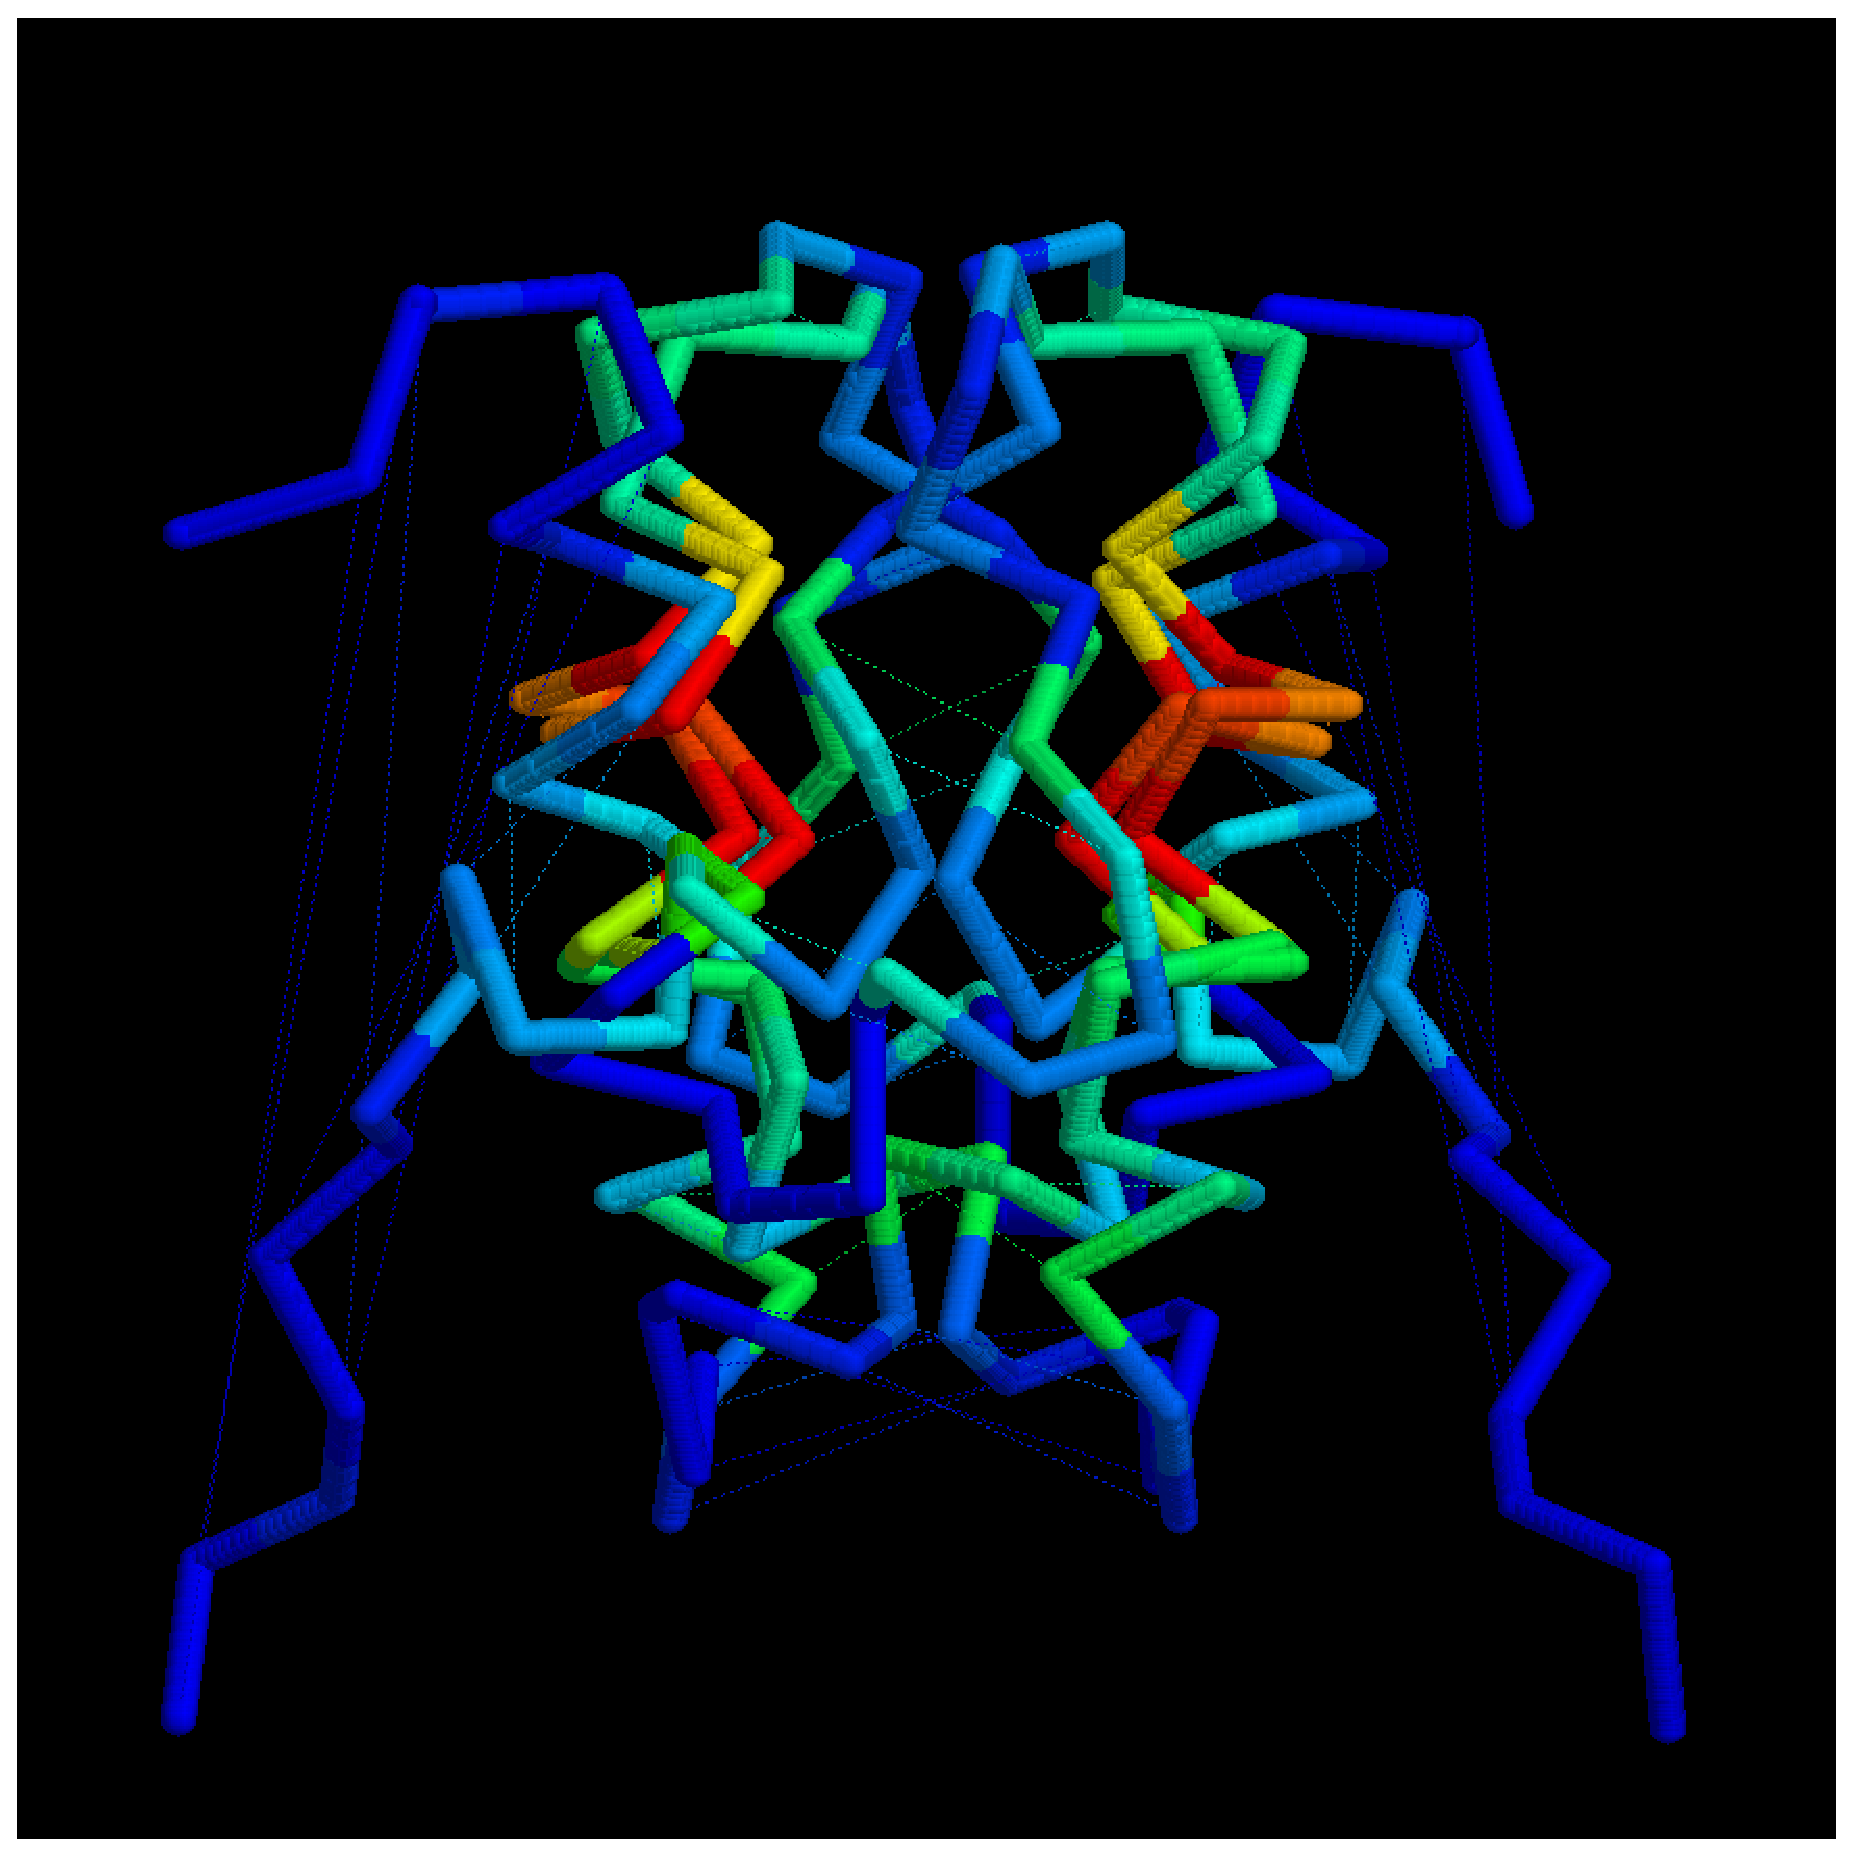
\includegraphics[width=150pt]{twoN.eps}
}
\subfigure[C]{
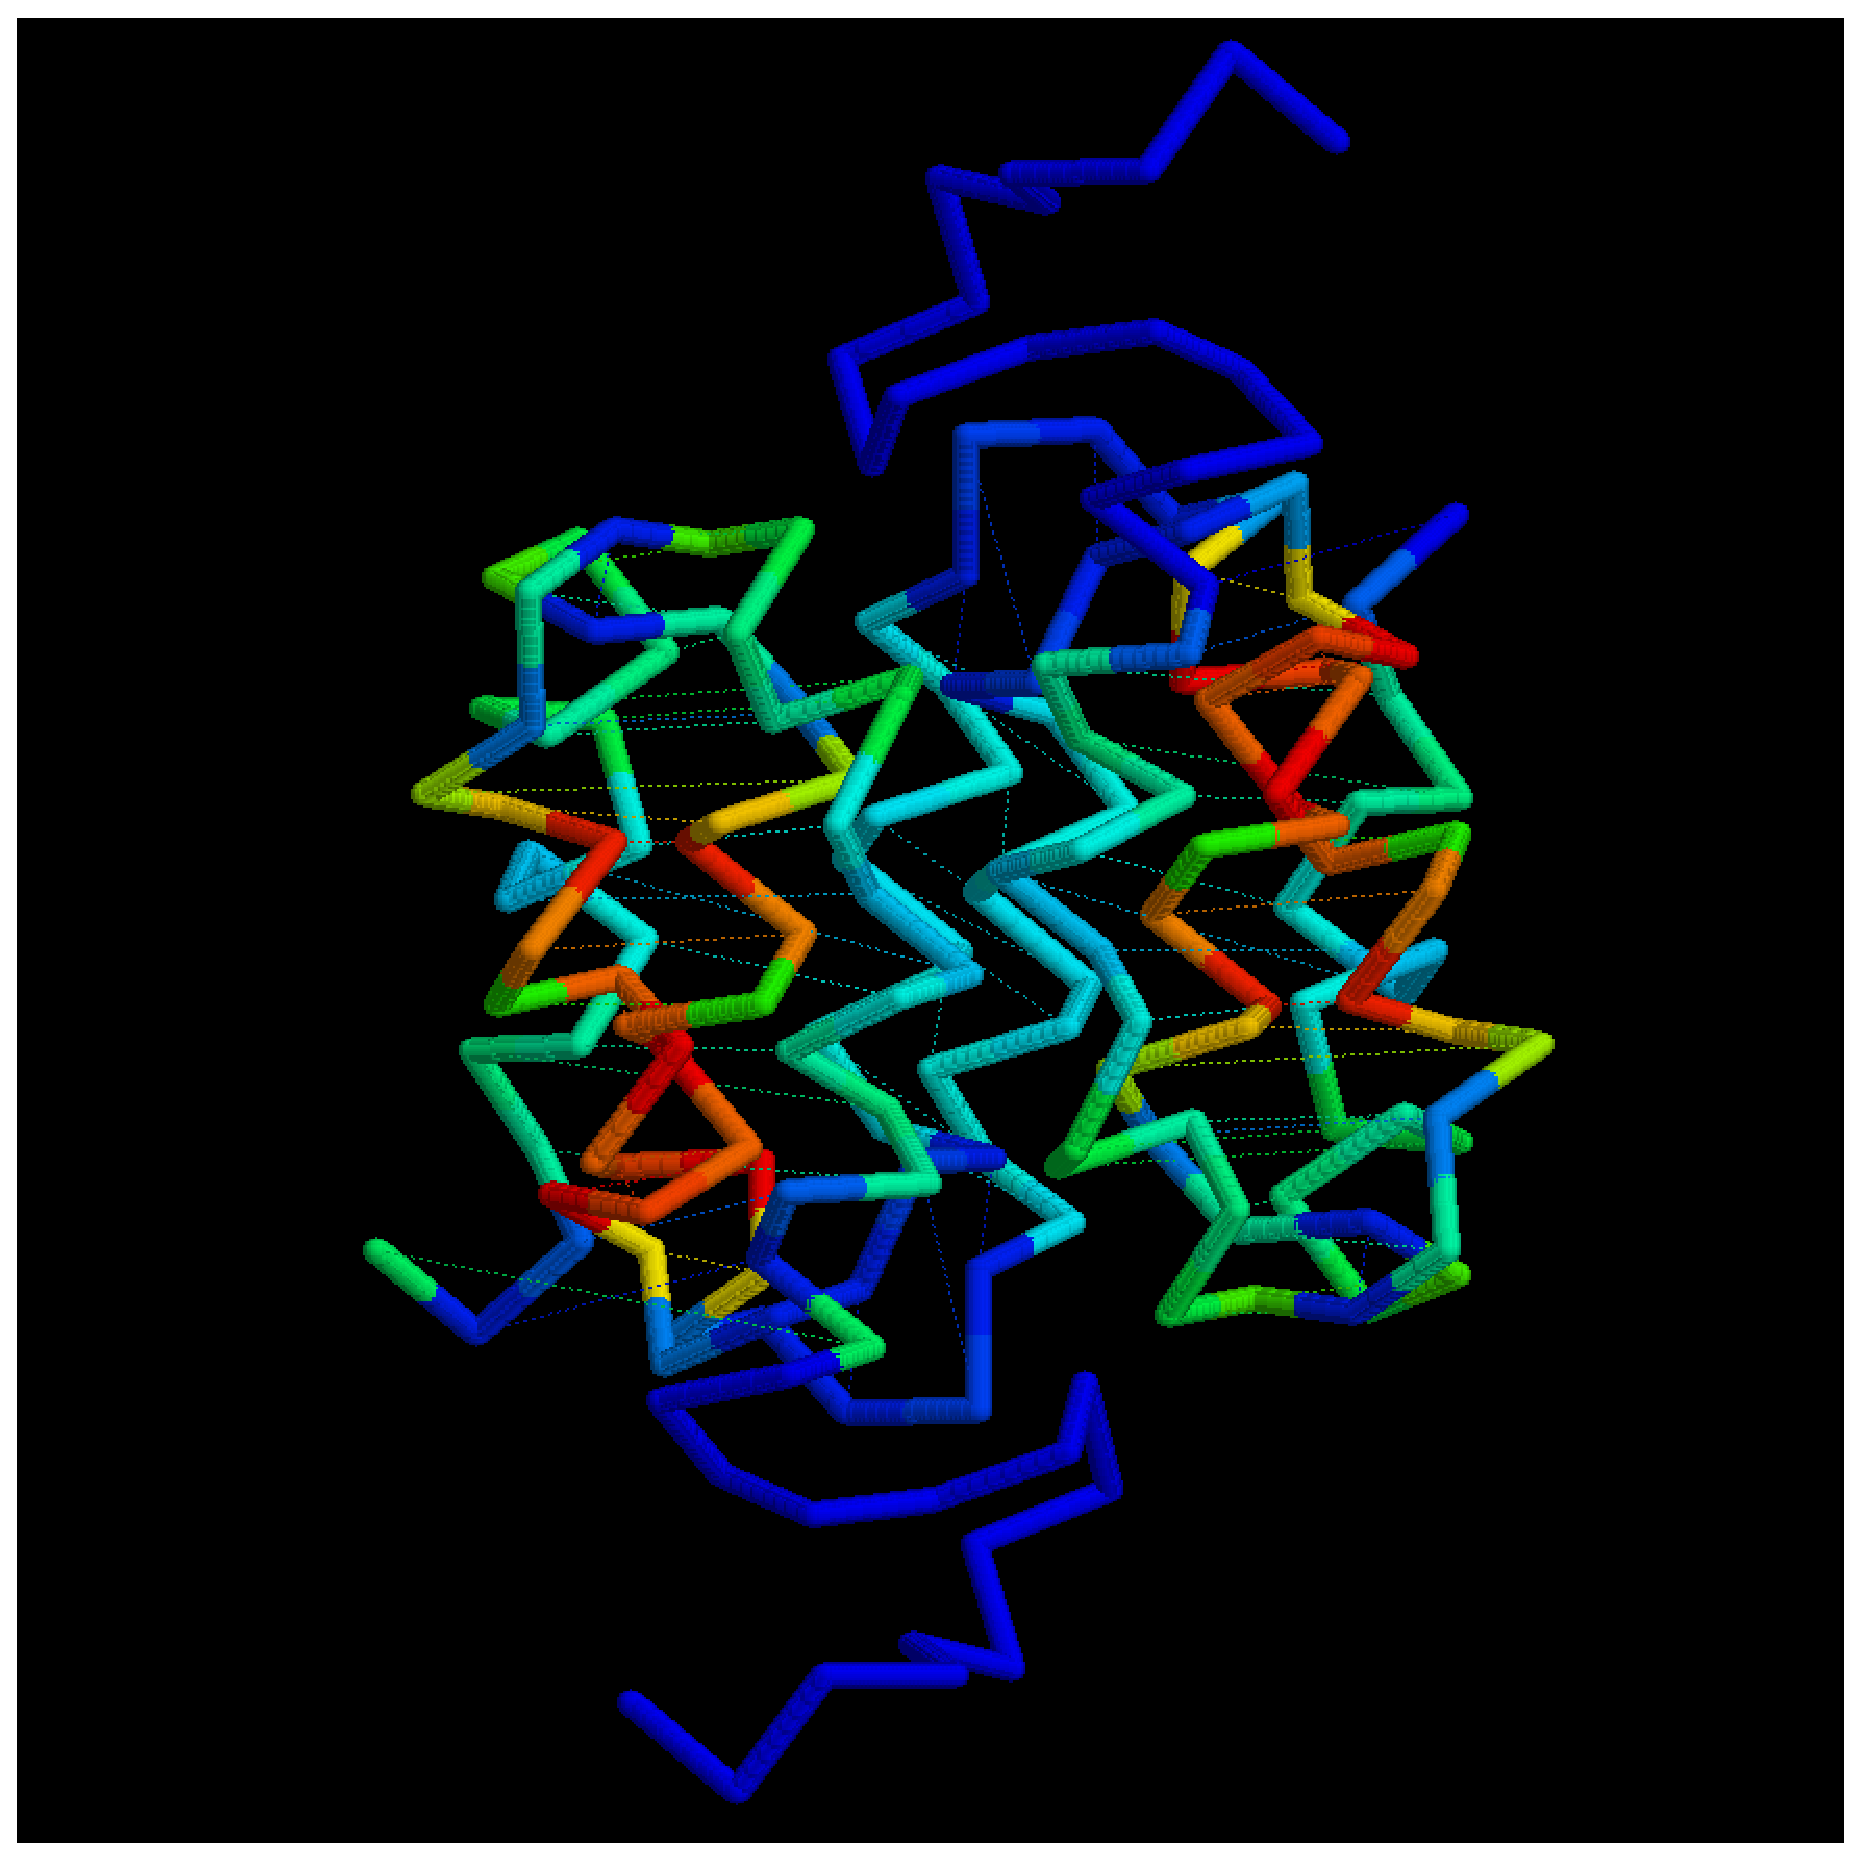
\includegraphics[width=150pt]{twoC.eps}
}
\begin{footnotesize}
\caption{
\label{Fig:tows}
{\bf Native/decoy similarity}.
When superposed using the program \SAP, both N-terminal (left) and C-terminal (right) domains
have some degree of similarity to their reversed decoy 'doppleganger', which is more marked
for the N domain.   The superposed structures are coloured by the \SAP\ residue-level score as
red = high similarity, blue = low.  The N domain has roughly 60 equivalent \CA\ positions
compared to only 24 in the larger C domain.
}
\end{footnotesize}
\end{figure}

\subsubsection{Customised decoy comparisons}

To improve the statistical analysis of the foamy/ortho capsid similarity, we employed a method
based on the generation of a population of customised 'decoy' models to provide a background distribution
of unrelated protein scores \cite{TaylorWR06a}.  This method retains the advantage of the simple
reversed structures where every comparison that constitutes the random pool is between two models
of the same size and secondary structure composition as the pair of native structures being compared.
For this study we collected 12 capsid N-terminal domains and 7 C-terminal domains, each of which
were compared with the foamy N-terminal domain and the foamy C-terminal domain.
(The structures are identified in Table 1 with full details in the Methods section).

For each domain pair to be compared, decoys were created using cyclic permutation and segment
swapping with chain reversal to generate a family of customised decoys for each comparison
\cite{TaylorWR06a}.  All pairs of forward/reversed decoys were then compared, with each pair being
drawn from a pool of models generated from the two native structures.  This ensures that the native
domains (which may have different lengths) are always evaluated against a decoy pair with the same
length combination.   (See Methods section for details).   All the decoy comparisons, of which
there are typically 150--300 for each comparison,  can then be compared to the native pair on a
plot of RMSD against the number of matched residues (\CA\ atoms).   An example is shown in
\Fig{sapit} for the comparison of the HIV1 structure (PDB codes: 1ak4 (N) and 1a43 (C)) domains
against the foamy virus gag domains.

\begin{figure}
\centering
\subfigure[orthoN+foamyN]{
\label{Fig:sapitNN}
\rotatebox{270}{
\includegraphics[width=130pt]{sapitNN.eps}
}}
\subfigure[orthoN+foamyC]{
\label{Fig:sapitNC}
\rotatebox{270}{
\includegraphics[width=130pt]{sapitNC.eps}
}}
\subfigure[orthoC+foamyN]{
\label{Fig:sapitCN}
\rotatebox{270}{
\includegraphics[width=130pt]{sapitCN.eps}
}}
\subfigure[orthoC+foamyC]{
\label{Fig:sapitCC}
\rotatebox{270}{
\includegraphics[width=130pt]{sapitCC.eps}
}}
\begin{footnotesize}
\caption{
\label{Fig:sapit}
{\bf ortho/foamy domains compared with customised decoys}.
Each amino (N), carboxy (C) domain combination between the ortho retrovirus capsid structure (HIV1)
and the foamy virus capsid structure is plotted as a line for increasingly large subsets of matched
positions against their RMSD (Y-axis), as in Figure 2.  The point on this line marks the lowest
$a$-value (\Eqn{fit}), however, to be consistent with the decoy data, the full alignment length
was used.  The decoy comparison data (blue) is plotted in a variety of symbols
with each representing a different combination of decoy construction.  The dashed blue lines
(which are the same in all plots) mark the approximate 10$^{th}$ percentile boundaries of
the decoy generated distributions,  with {\tt a} = 1.7 (upper) and  {\tt a} = 0.8 (lower).
(See Methods section for details).
}
\end{footnotesize}
\end{figure}

\begin{figure}
\centering
\subfigure[]{
\label{Fig:normHIV}
\rotatebox{270}{
\includegraphics[width=130pt]{fitsCN-plothiv.eps}
}}
\subfigure[]{
\label{Fig:normALL}
\rotatebox{270}{
\includegraphics[width=130pt]{fitsCN-plotall.eps}
}}
\begin{footnotesize}
\caption{
\label{Fig:norms}
{\bf ortho-C and foamy-N domain comparison statistics}.
The $a$-value (normalised RMSD) for the comparison of the ortho-C and foamy-N decoy domains
(Figure 8($b$)) are plotted as a frequency distribution (red) along with a bell-shaped
Normal distribution curve (green) with matching mean ($\mu$) and spread ($\sigma$).
Part ($a$) shows the distribution for the HIV1 C-terminal domain ($\mu = 1.23$) and spread ($\sigma = 0.17$)
with the position of the native structure comparison plotted as a blue (inverted) triangle.
Its position lies 0.64 units below the mean giving a Z-score of $0.64/0.17 = 3.76$.
Part ($b$) shows the combined data from seven representative viruses (in Table 1).
These data comprise two distributions, that of the combined decoys and also the much smaller
distribution of native scores (blue triangles).   This allows a T-test to be made on the
significance of their separation.
}
\end{footnotesize}
\end{figure}

\subsubsection{Statistical analysis of the decoy comparisons}

The quality of the comparisons in \Fig{sapit} can be quantified as a combination of their
RMSD ($R$) and the number of matched (superposed) positions ($N$).   However, as explained in
the Methods section, for statistical analysis, it is easier to combine this pair of numbers
as a single number,  called the $a$-value (\Eqn{fit}), which is the scaling factor that
causes a theoretical curve to pass through the point ($R,N$).

When expressed by a single $a$-value
all the data points in a comparison, such as \Fig{sapitCN},
can be plotted as a frequency histogram and examined to see if they approximate a Normal
distribution.   The distributions were found to be a good fit to unskewed Gaussians and
so were treated as normal distributions (rather than extreme value distributions
that have also been considered previously as a model for random structure comparison scores
\cite{LevittMet98,TaylorWR06a}).    The frequency data from the comparison of the orthoN domain from
HIV1 and the foamyC domain (\Fig{sapitCN}) is shown in \Fig{normHIV} along with a Normal
distribution that has the same mean ($\mu$) and standard deviation ($\sigma$) as the data.
On this plot, the value of $a$ (\Eqn{fit}) for the comparison of the
native pair of domains is also plotted (blue triangle) and from its position, a Z-score
can be calculated.

In this way, the significance of all combinations of the native ortho and foamy domain
superpositions were calculated, using the background distribution of 'customised' decoy
comparisons based on each individual native pair.   The resulting Z-scores ($\sigma$ units)
are collected in \Tab{Zscores}.   The degree of similarity between the domains ranged from
less than 1$\sigma$ to over 5$\sigma$, with the latter (highly significant) result being
obtained for both a swapped (NC) and forward (CC) combination.   However, of the top 12
scores, only three now came from swapped pairings.

\begin{table}
\centering
\begin{tabular}{r|lll|lll|}
$a$  & \multicolumn{6}{c|}{\bf ortho-N} \\
     & \multicolumn{3}{c|}{\bf foamy-N} & \multicolumn{3}{c|}{\bf foamy-C}  \\
\hline \hline
virus  & pool & $a$-value & Z-score & pool & $a$-value & Z-score \\
\hline
BLV6   &  300  & 0.552 & {\bf 4.073} &  244  & 0.542 &      3.692  \\
BLV    &  251  & 0.550 & {\bf 4.494} &  184  & 0.400 &      3.669  \\
HIV6   &  312  & 0.551 &      3.781  &  220  & 0.405 &      3.579  \\
HIV1   &  312  & 0.573 &      3.703  &  213  & 0.402 &      3.692  \\
HML2   &  264  & 0.777 &      2.166  &  196  & 0.438 & {\bf 4.594} \\
HTLV   &  400  & 0.592 & {\bf 4.030} &  328  & 0.457 & {\bf 4.013} \\
JSRV   &  225  & 1.063 &      0.896  &  190  & 0.601 &      3.237  \\
MLV    &  326  & 0.751 &      3.044  &  188  & 0.508 &      3.151  \\
MPMV   &  269  & 0.565 & {\bf 3.902} &  185  & 0.523 &      2.918  \\
PSIV   &  285  & 0.621 &      3.731  &  235  & 0.369 & {\bf 5.019} \\
RELIK  &  234  & 0.639 &      3.688  &  237  & 0.700 &      3.297  \\
RSV    &  204  & 0.543 &      3.123  &  239  & 0.526 &      3.542  \\
\hline \hline
\vspace{10pt}
\end{tabular}
\begin{tabular}{r|lll|lll|}
$b$  & \multicolumn{6}{c|}{\bf ortho-C} \\
     & \multicolumn{3}{c|}{\bf foamy-N} & \multicolumn{3}{c|}{\bf foamy-C}  \\
\hline \hline
virus  & pool & $a$-value & Z-score & pool & $a$-value & Z-score \\
\hline
BLV6   &  144  & 0.763 &      3.019  &  212  & 0.709 & {\bf 4.046} \\
BLV    &  154  & 0.578 &      3.400  &  204  & 0.556 & {\bf 4.047} \\
HIV1   &  157  & 0.593 &      3.760  &  174  & 0.705 &      3.362  \\
HIV6   &  179  & 0.780 &      3.175  &  177  & 0.640 & {\bf 4.380} \\
HML2   &  185  & 0.732 &      3.027  &  184  & 0.676 & {\bf 3.900} \\
HTLV   &  156  & 0.685 &      3.847  &  163  & 0.694 &      2.807  \\
RSV    &  155  & 0.448 &      3.754  &  235  & 0.403 & {\bf 5.009} \\
\hline \hline
\end{tabular}
\begin{footnotesize}
\caption{
\label{Tab:Zscores}
{\bf Ortho and foamy domain comparison Z-score statistics}.
For each amino (N) and carboxy (C) domain pair between an ortho virus structure and the foamy virus capsid structure,
a {\bf Z-score} is calculated based on the {\bf a-value} (\Eqn{fit}) derived from the comparison RMSD and length,
relative to the {\bf pool} of background decoy comparisons.   The ortho {\bf virus} identity is indicated by the
code to the left, full details of which can be found in the Methods section.
The top 12 Z-scores are high-lighted in bold, only three of which support a swapped domain match.
}
\end{footnotesize}
\end{table}

\paragraph{Asymmetry statistics:}\

To quantify the degree of bias for domains of like-type (NN, CC) to be more similar than those of mixed-type (NC, CN),
the observed ranking of like and mixed pairs, based on their Z-value (\Tab{Zscores}), was compared to that expected by
chance.  The positions of all pairs in the list were shuffled a million times and the asymmetry of each arrangement was
quantified as the number of like-pairs in the top half and also by their second moment: $\surd((\sum r^2_i)/N)$, where $r$
is the rank of the like-pair $i$ in a list of $N$ pairs.  The chance of obtaining a distribution with more like-pairs
being ranked higher can be caluclated by summing the area of the tail of each empirical distribution that lies beyond the
observed value.   However, these values were calculated over all pairs and neglects the principle that emphasis should
be given to the more significant similarities.  Rather than rely on a single significance cutoff (like 3$\sigma$) or an
arbitrary cutoff (like the "3-out-of-12" mentioned above), we calculated statistics for all such cutoffs (\Fig{splitALL}).

\begin{figure}
\centering
\subfigure[Full data set]{
\label{Fig:splitALL}
\rotatebox{270}{
\includegraphics[width=130pt]{splitALL.eps}
}}
\subfigure[5N+5C data set]{
\label{Fig:split5+5}
\rotatebox{270}{
\includegraphics[width=130pt]{split5+5.eps}
}}
\begin{footnotesize}
\caption{
\label{Fig:splits}
{\bf Asymmetry statistics for like/mixed domain pairs}.
Given the ranked list of domain pairings, the chance for more domain pairs of like-type
to be found higher than the observed order was evaluated from empirical distributions
measured by two statistics: the second moment of the rank value (red) and the number
of like-type pairs in the top half (blue).   These statistics were calculated for all
subsets from the 6 top pairs up to the full set of comparisons (X-axis) and for each,
the chance of a better score is plotted as the log$_{10}$ of the probability (Y-axis).
The horizontal lines mark the 0.5, 0.05 and 0.005 levels.
The line at the 0.001 level is coloured by the Z-score for each pair as: green = over 3
and cyan = over 4 sigma.
Part ($a$) shows the probabilities calculated from the full set of 7 carboxy and 12
amino domains and part ($b$) shows the same values calculated on a more balanced
set of 5 non-redundant carboxy domains and their matching amino domains.
}
\end{footnotesize}
\end{figure}

The majority of values in \Fig{splitALL} lie below the 0.05 probability level for the larger sample sizes,
with those for the top-half bias statistic (blue line) being more significant than the moment-based statistic (red line).
While confirming the visual trend towards a bias of higher scoring like-type domain similarities, the analysis
summarised in \Fig{splitALL} is complicated by having unequal numbers of amino and carboxy domain comparisons
and also by including some closely related structures.   To produce a more balanced data-set, one of each
pair of the two most similar carboxy domain structures was discarded leaving five structures and for each
of these, their matching amino terminal domain was also retained, leaving: BLV-1, HIV-1, HML2, HTLV-1 and RSV.
Despite having a smaller set of comparisons
(5N + 5C domains giving 20 rather than 38 Z-scores), the results for this reduced set indicated
an equally clear bias towards towards a preferred like-domain equivalance, especially as measured by their
occurrence in the upper half of the ranked list, with several having a probability below the 0.05 level and
a few below the 0.005 level (\Fig{split5+5}).

\paragraph{T-test statistic:}\

An alternative to the above analysis, which still remains marginally significant, is to
pool the raw comparison data for all the domain comparisons and their background distributions
giving now not just a single value compared to a distribution but two distributions (\Fig{normALL}).
For these data, a significance was calculated using Student's T-test, the values of which are given
in \Tab{Ttest}.

\begin{table}
\centering
\begin{tabular}{c|c|c|}
             &          {\bf orthoN}           &          {\bf orthoC}           \\
\hline \hline
             & {\tt Avg: 6.67e-01 < 1.32e+00 } & {\tt Avg: 6.51e-01 < 1.25e+00 } \\
             & {\tt Tprob = 4.62e-21 **      } & {\tt Tprob = 2.35e-16 **      } \\
{\bf foamyN} &                                 &                                 \\
             & {\tt StD: 1.61e-01 = 2.12e-01 } & {\tt StD: 1.17e-01 = 1.89e-01 } \\
             & {\tt Fprob = 1.84e-01         } & {\tt Fprob = 1.12e-01         } \\
\hline
             & {\tt Avg: 4.92e-01 < 1.29e+00 } & {\tt Avg: 6.22e-01 < 1.30e+00 } \\
             & {\tt Tprob = 4.09e-10 **      } & {\tt Tprob = 3.81e-23 **      } \\
{\bf foamyC} &                                 &                                 \\
             & {\tt StD: 1.02e-01 < 2.21e-01 } & {\tt StD: 1.12e-01 = 1.77e-01 } \\
             & {\tt Fprob = 7.37e-03 **      } & {\tt Fprob = 1.20e-01         } \\
\hline \hline
\end{tabular}
\begin{footnotesize}
\caption{
\label{Tab:Ttest}
{\bf ortho and foamy capsid domain comparison T-test significance}.
For each combinfation of domains between the ortho and foamy viruses, the probability
is given that the two means from each distribution ({\tt Avg} values) were sampled
from the same distribution.  (i.e., that the native and decoy comparisons are
not distinct).   All domain pairings are extremely significant.   An F-test was used to
test if the standard deviations ({\tt Std}) of each sample were distinct and if not,
the a T-test was made on the assumption of equal standard deviations.
}
\end{footnotesize}
\end{table}

From these results, it can be seen that all the four possible pairings are
highly significant with probabilities ranging from $10^{-10}$ to over $10^{-20}$.
It is also clear that the two swapped pairings (NC and CN) have higher probabilities
than the forward pairings (NN and CC).   Combining the probabilities ($P$) as:
$\Delta P = \log_{10}(P_{NN} P_{CC}) - log_{10}(P_{NC} P_{CN})$,
gives a value of 17.7 (42.7 - 25.0) which means that the swapped pairing is almost 18
orders of magnitude less likely than the forward pairing.
Calculating the same statistic on the reduced 5N+5C domain data set gave a similar result
but with a difference reduced 1000-fold to 15 orders of magnitude.

The unexpected swapped pairing, which was indicated originally by the \DALI\ results, now seems
less likely.  The preferred, and biologically more reasonable, result is that the ortho virus
domain are related to the foamy virus domains as a result of genetic divergence from
a common, double domain ancestor.

\subsection{Internal duplication}

The transposed pairings of N/C and C/N (ortho/foamy) domains still retain a high structural
significance and this suggests that the two domains are derived from a common ancestral structure,
probably as the result of a prior gene-duplication event that has been retained more clearly
in the less embellished foamy virus structures.   Comparing the two foamy domains gives
a Z-score of 2.077 sigma which, although of marginal significance, supports this model.
(\Fig{fitsNC}($a,b$)).

Such a relationship between the foamy domains implies an equivalent relationship
in the ortho viruses and a similar comparison in structures of their N and C domains
finds matches with Z-scores ranging from 2 to 4.   As with the comparison of the
ortho and foamy structures, these can be pooled to allow a joint T-test to be applied.
This gave a probability of $10^{-8}$ that the true N/C domain
comparisons were drawn from the decoy distribution, adding strong support to the
hypothesis of an ancient gene duplication occurring before the split of the ortho
and foamy virus families. (\Fig{fitsNC}($c,d$), blue triangles).
Supporting this relationship, earlier studies also sugggested an internal duplication
in the ortho virsuses but were based largely on very distant sequence similarity
\cite{CampillosMet06}.

This test was applied only to the comparison of domains between viruses with
known structures for both domains, however, it is not unreasonable to compare
amino and carboxy domains across all viruses.  The longer loops in the ortho virus
domains gives greater scope of structural variation and a wide range of variation
was seen ranging from RMSD values under 4 to over 12.
When normalised for length ($a$-value from \Eqn{fit}) and partial matches under
60 positions excluded, a distinct cluster remains between $a=0.5\ldots0.8$ (4...6\AA\
RMSD) but still with a long tail to higher values.
Despite this tail, the T-test on the distributions is highly significant at $2.7 \times 10^{-17}$.

One of the better N/C ortho similarities is shown in \Fig{final}($a$), along with the
N/C ortho domain superposition in \Fig{final}($b$).

\begin{figure}
\centering
\subfigure[foamy N+C]{
\label{Fig:foamyNCsapit}
\rotatebox{270}{
\includegraphics[width=130pt]{foamyNC-sapit.eps}
}}
\subfigure[foamy fit]{
\label{Fig:foamyNCfits}
\rotatebox{270}{
\includegraphics[width=130pt]{foamyNC-fits.eps}
}}
\subfigure[ortho N+C]{
\label{Fig:orthoNCsapit}
\rotatebox{270}{
\includegraphics[width=130pt]{orthoNCall-sapit.eps}
}}
\subfigure[ortho fit]{
\label{Fig:orthoNCfits}
\rotatebox{270}{
\includegraphics[width=130pt]{orthoNCall-fits.eps}
}}
\begin{footnotesize}
\caption{
\label{Fig:fitsNC}
{\bf N and C domains compared with customised decoys}.
$a$) The N and C domains of the foamy virus (black) compared to decoys (blue) with ($b$) the derived frequency plot with the
native comparison marked by a blue triangle.  (See legend to \Fig{sapit} for details).
$c$) The N and C domains of the ortho virus combinations (black) with ($d$) the derived frequency plot showing the
native comparison for pairs from the same virus (blue triangles) with the distribution of all native pairs
shown as a scattered frequency plot (blue line).
(See Methods section for details).
}
\end{footnotesize}
\end{figure}

\begin{figure}
\centering
\subfigure[ortho]{
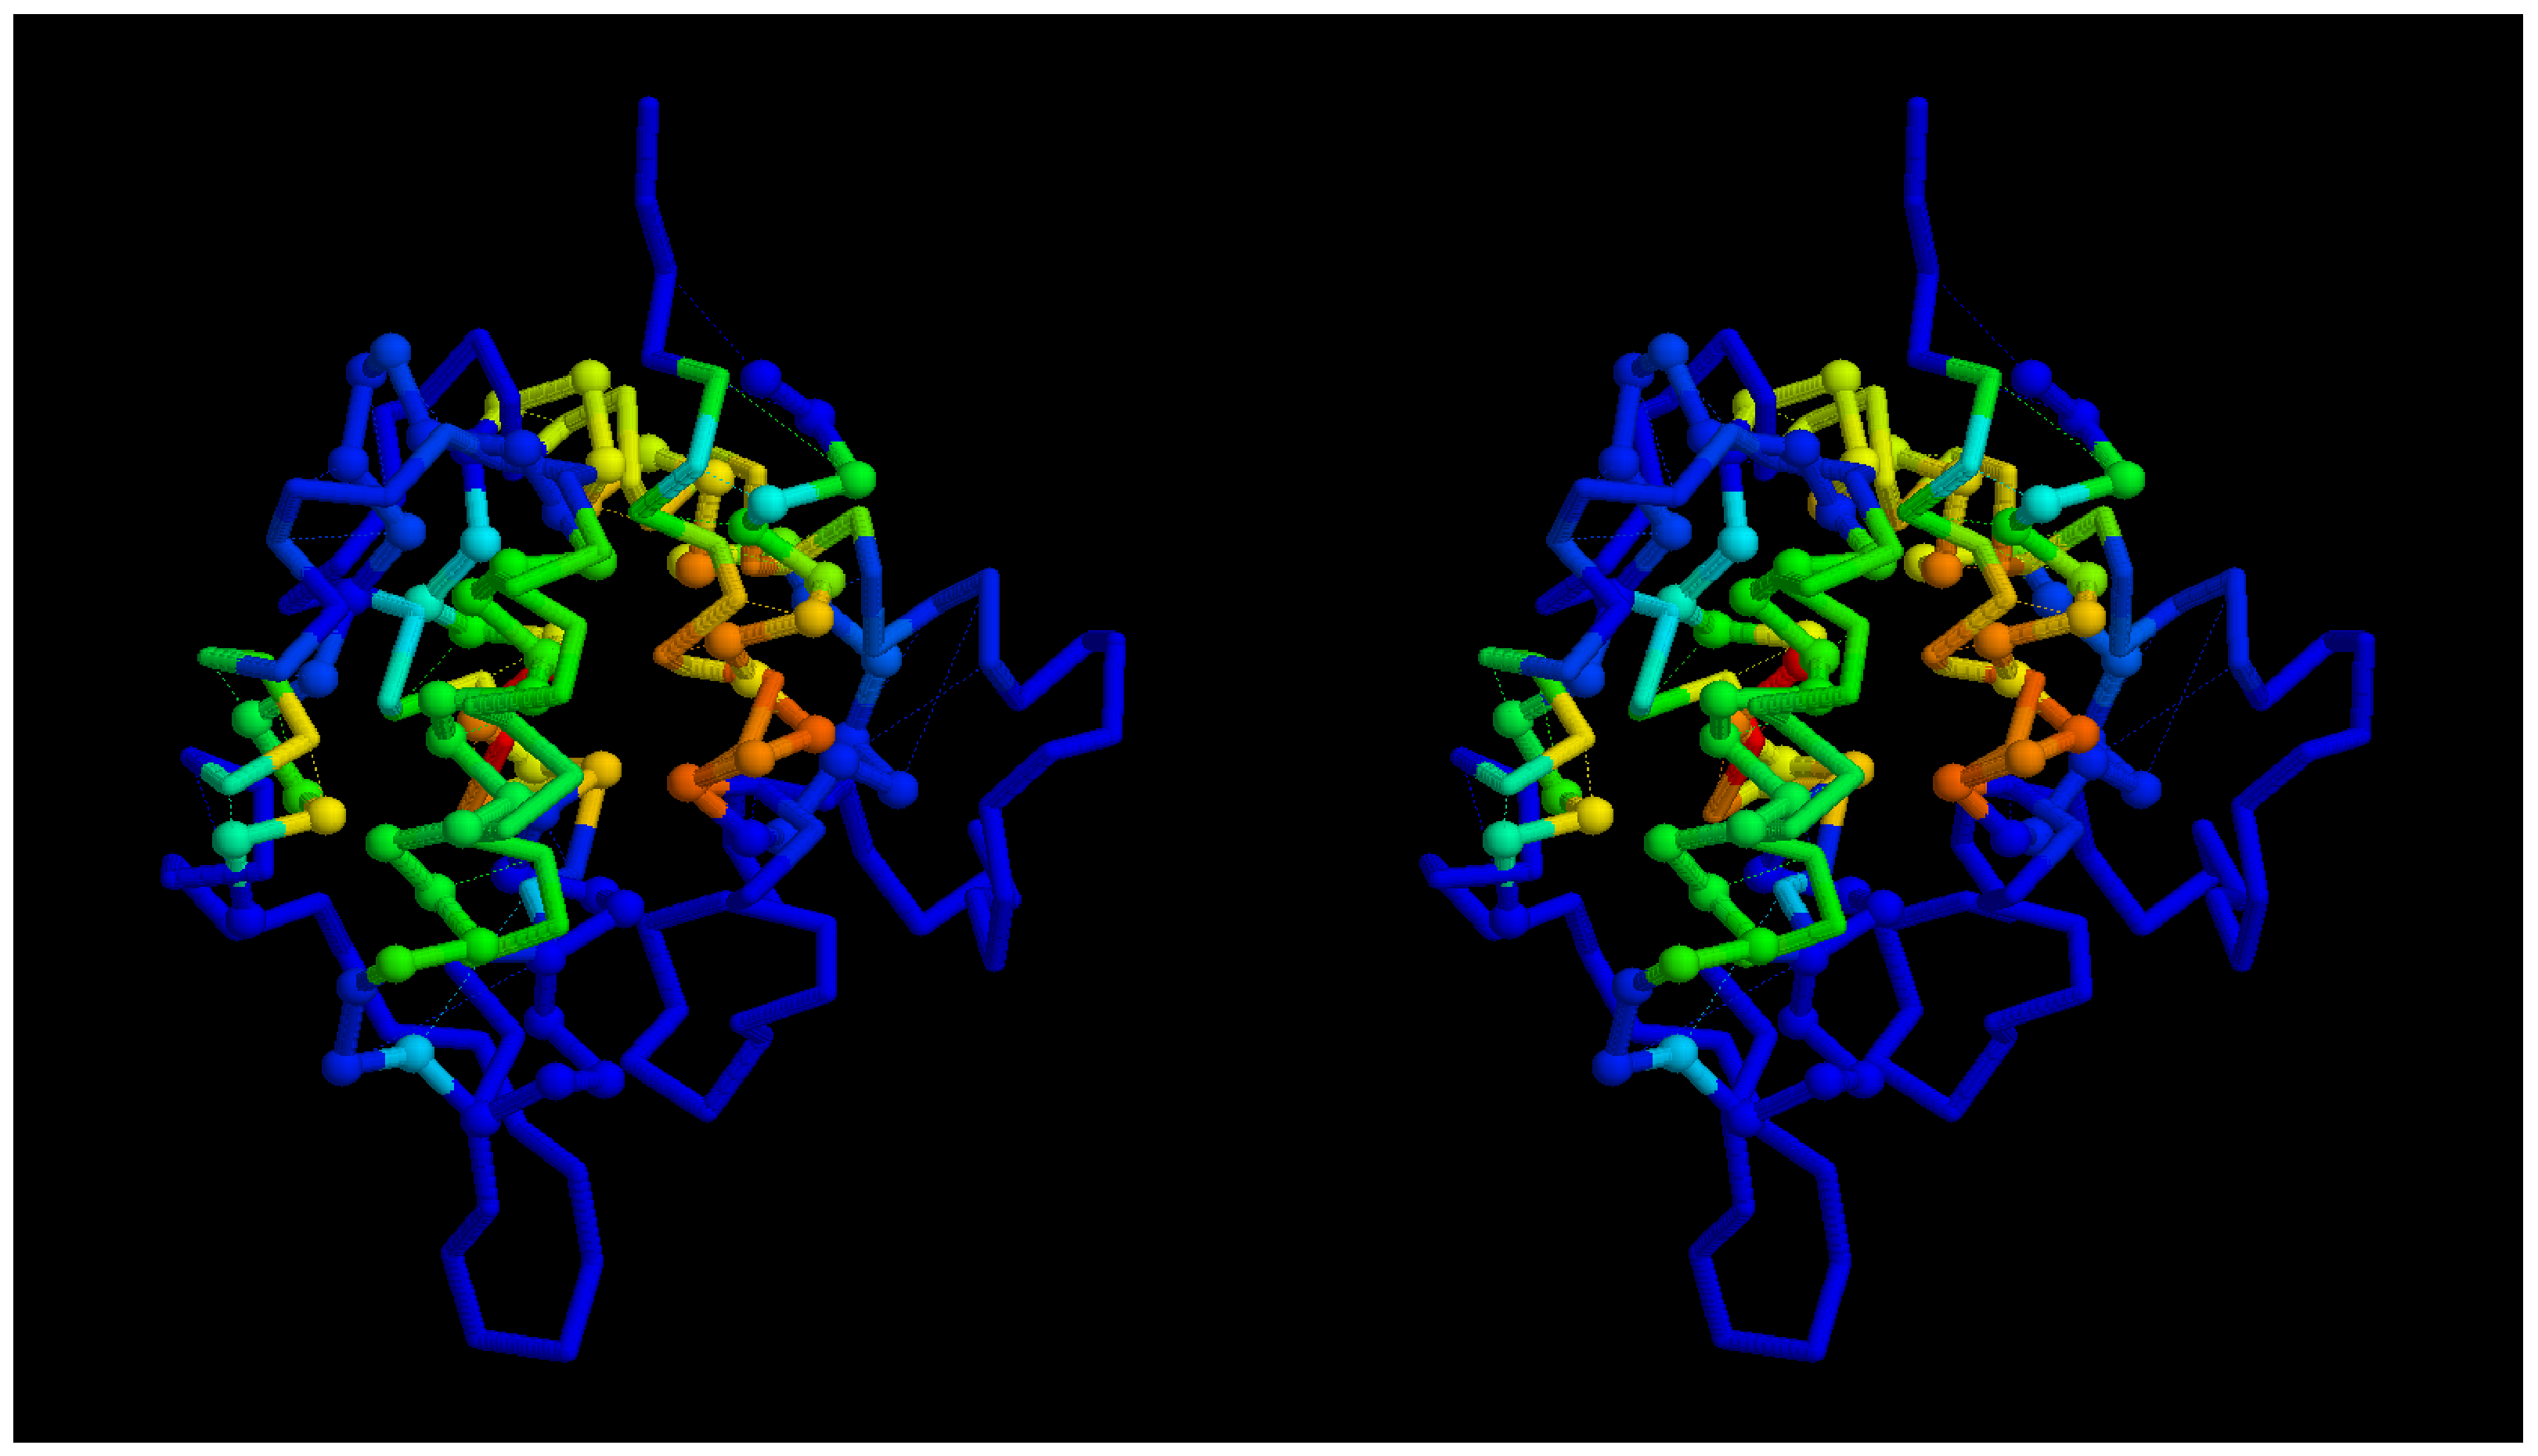
\includegraphics[width=300pt]{orthoNCall-ortho.eps}
}
\subfigure[foamy]{
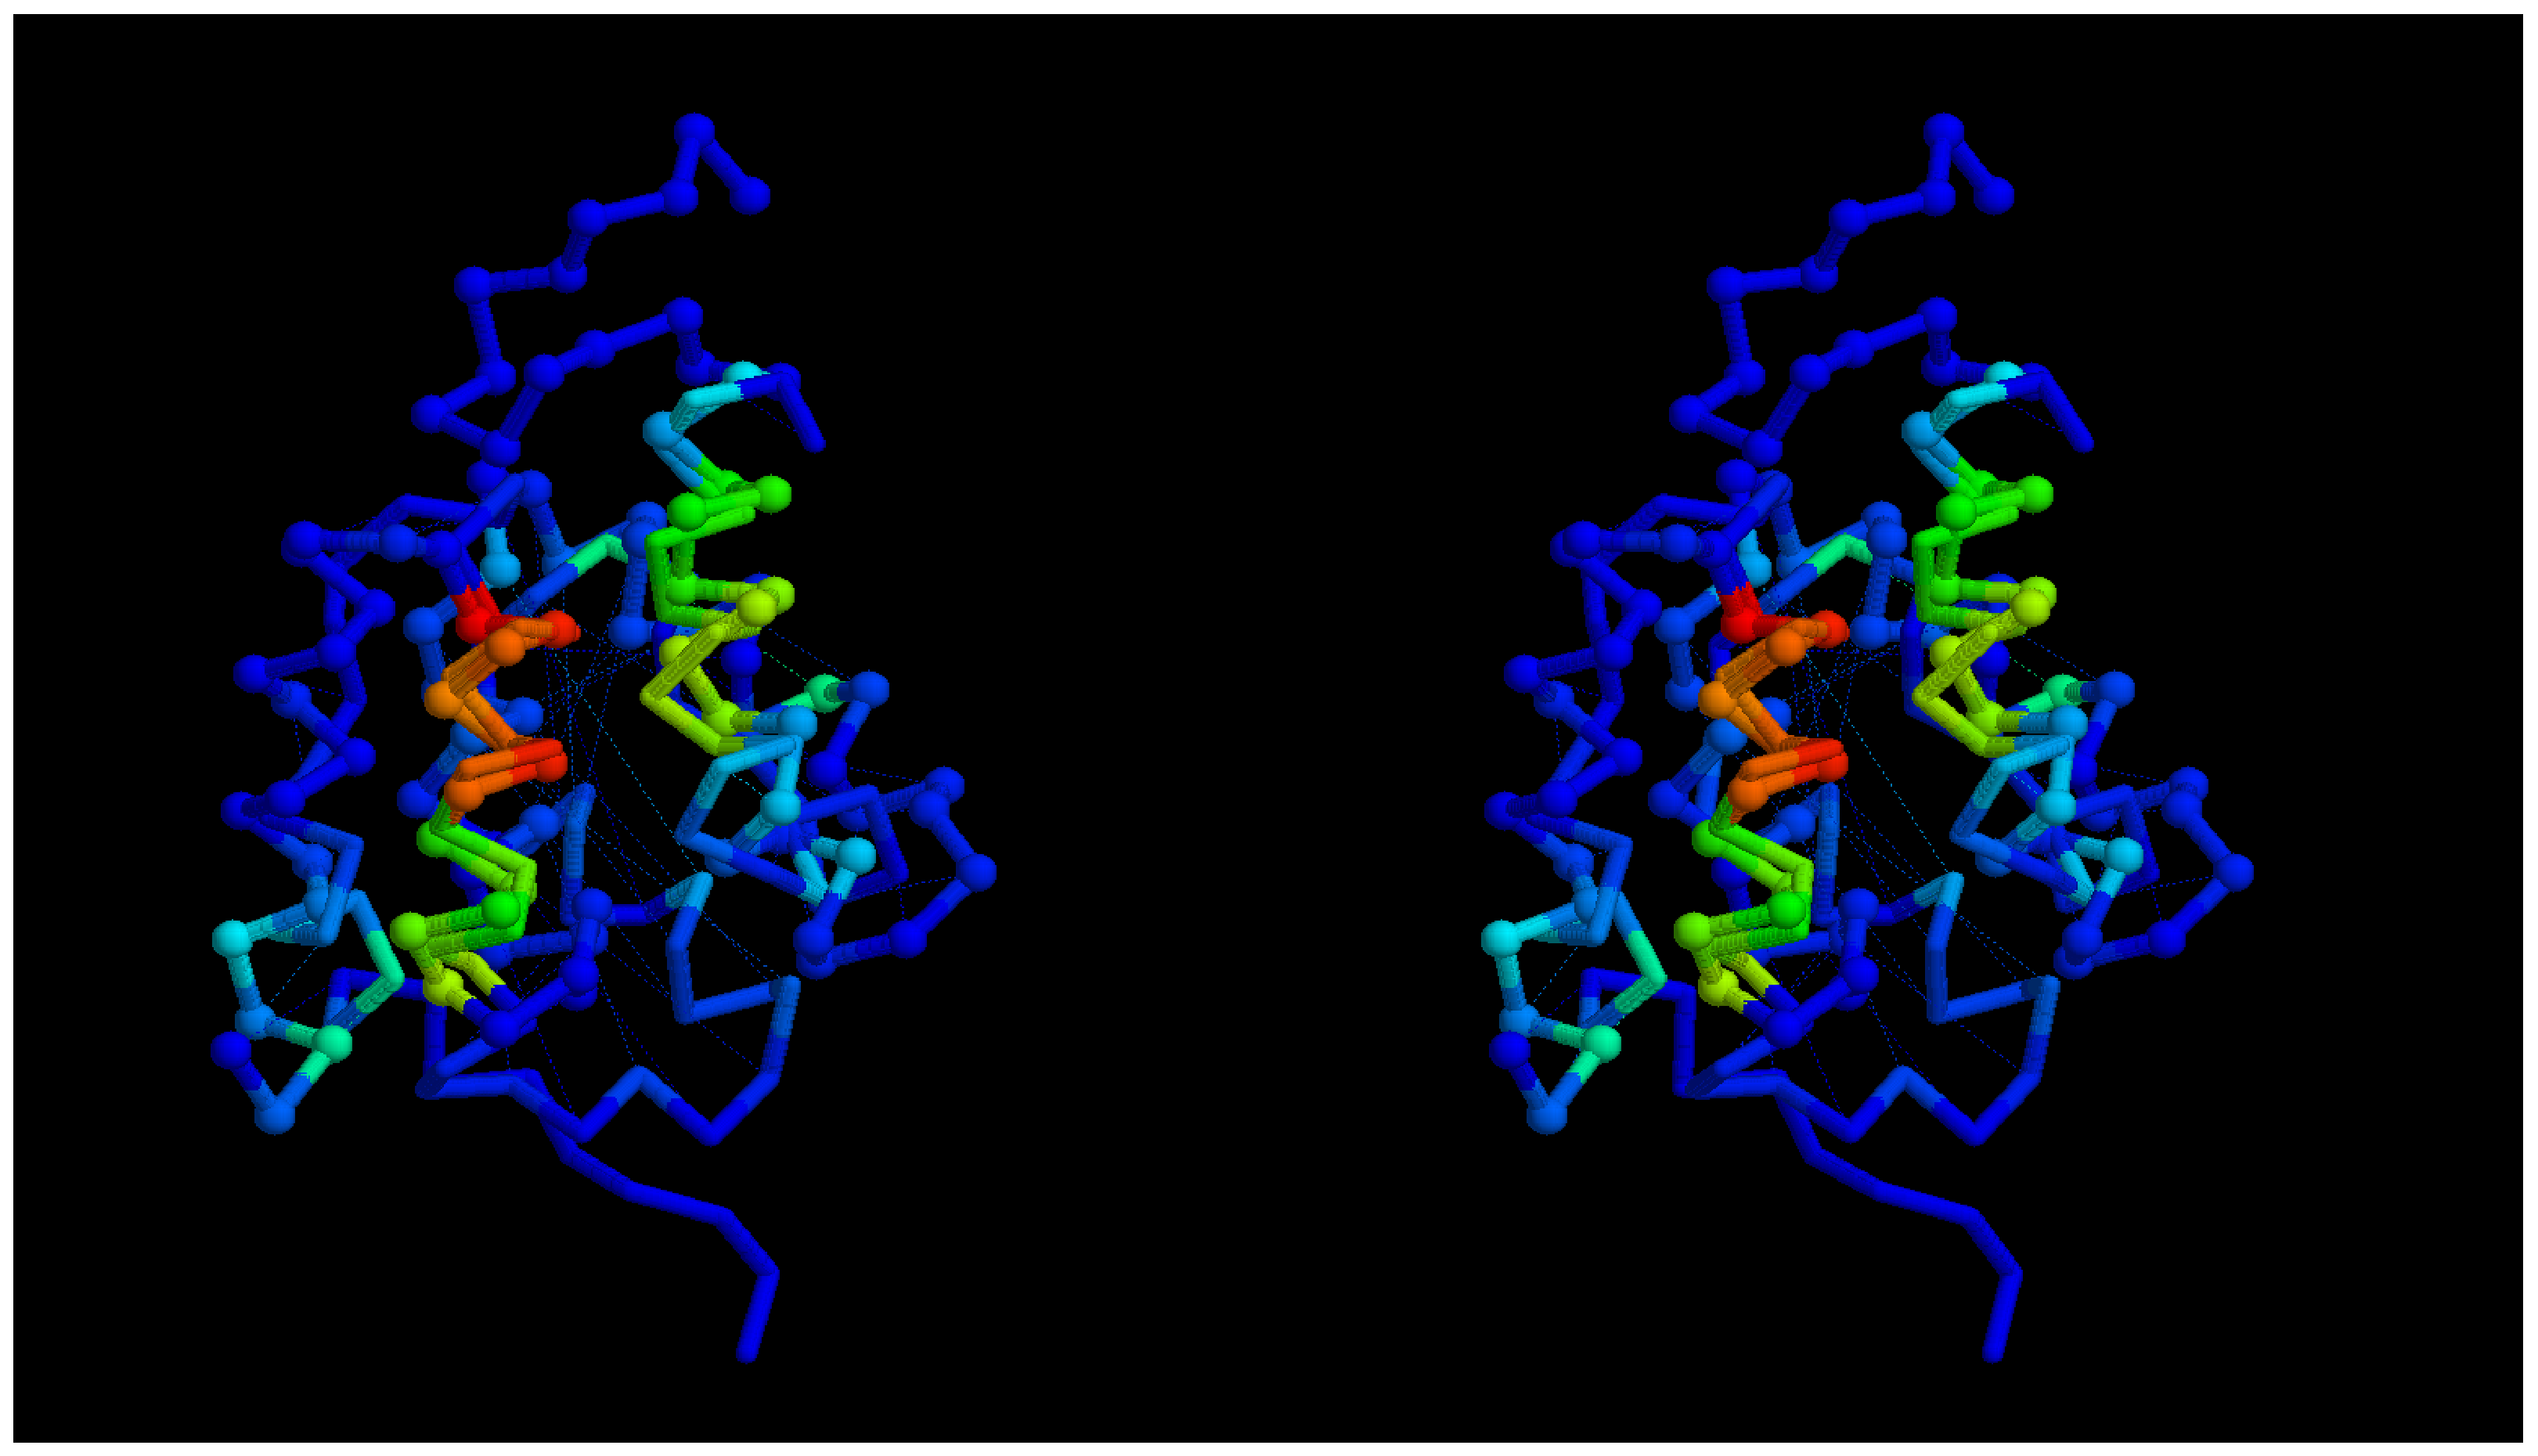
\includegraphics[width=300pt]{orthoNCall-foamy.eps}
}
\begin{footnotesize}
\caption{
\label{Fig:final}
{\bf Amino and carboxy domains superposed}.
$a$ ortho virus domains and
$b$ foamy virus domains are shown as a stereo pair with
their \CA\ backbones coloured by
the residue similarity score calculated by \SAP. (red = strong similarity, blue = none).
The amino terminal domain is distinguished by small balls on its \CA\ positions and
the amino terminus lies to the top in both panels.
}
\end{footnotesize}
\end{figure}

\subsection{Fold-space representation}

To summarise the structural relationships among the ortho and foamy domains, the matrix
of pairwise comparisons was projected into a three-dimensional fold-space.  (See methods
for details).   This produces a best visual representation of the RMSD values between domains.

As can be seen from \Fig{space}, the N and C domains of the ortho viruses form distinct
clusters with the foamy C domain lying closer to the ortho C-domain cluster.   The foamy
N-domain, however, maintains a fairly equal distance from both ortho domain clusters but
lies closer to its C-terminal partner.

\begin{figure}
\centering
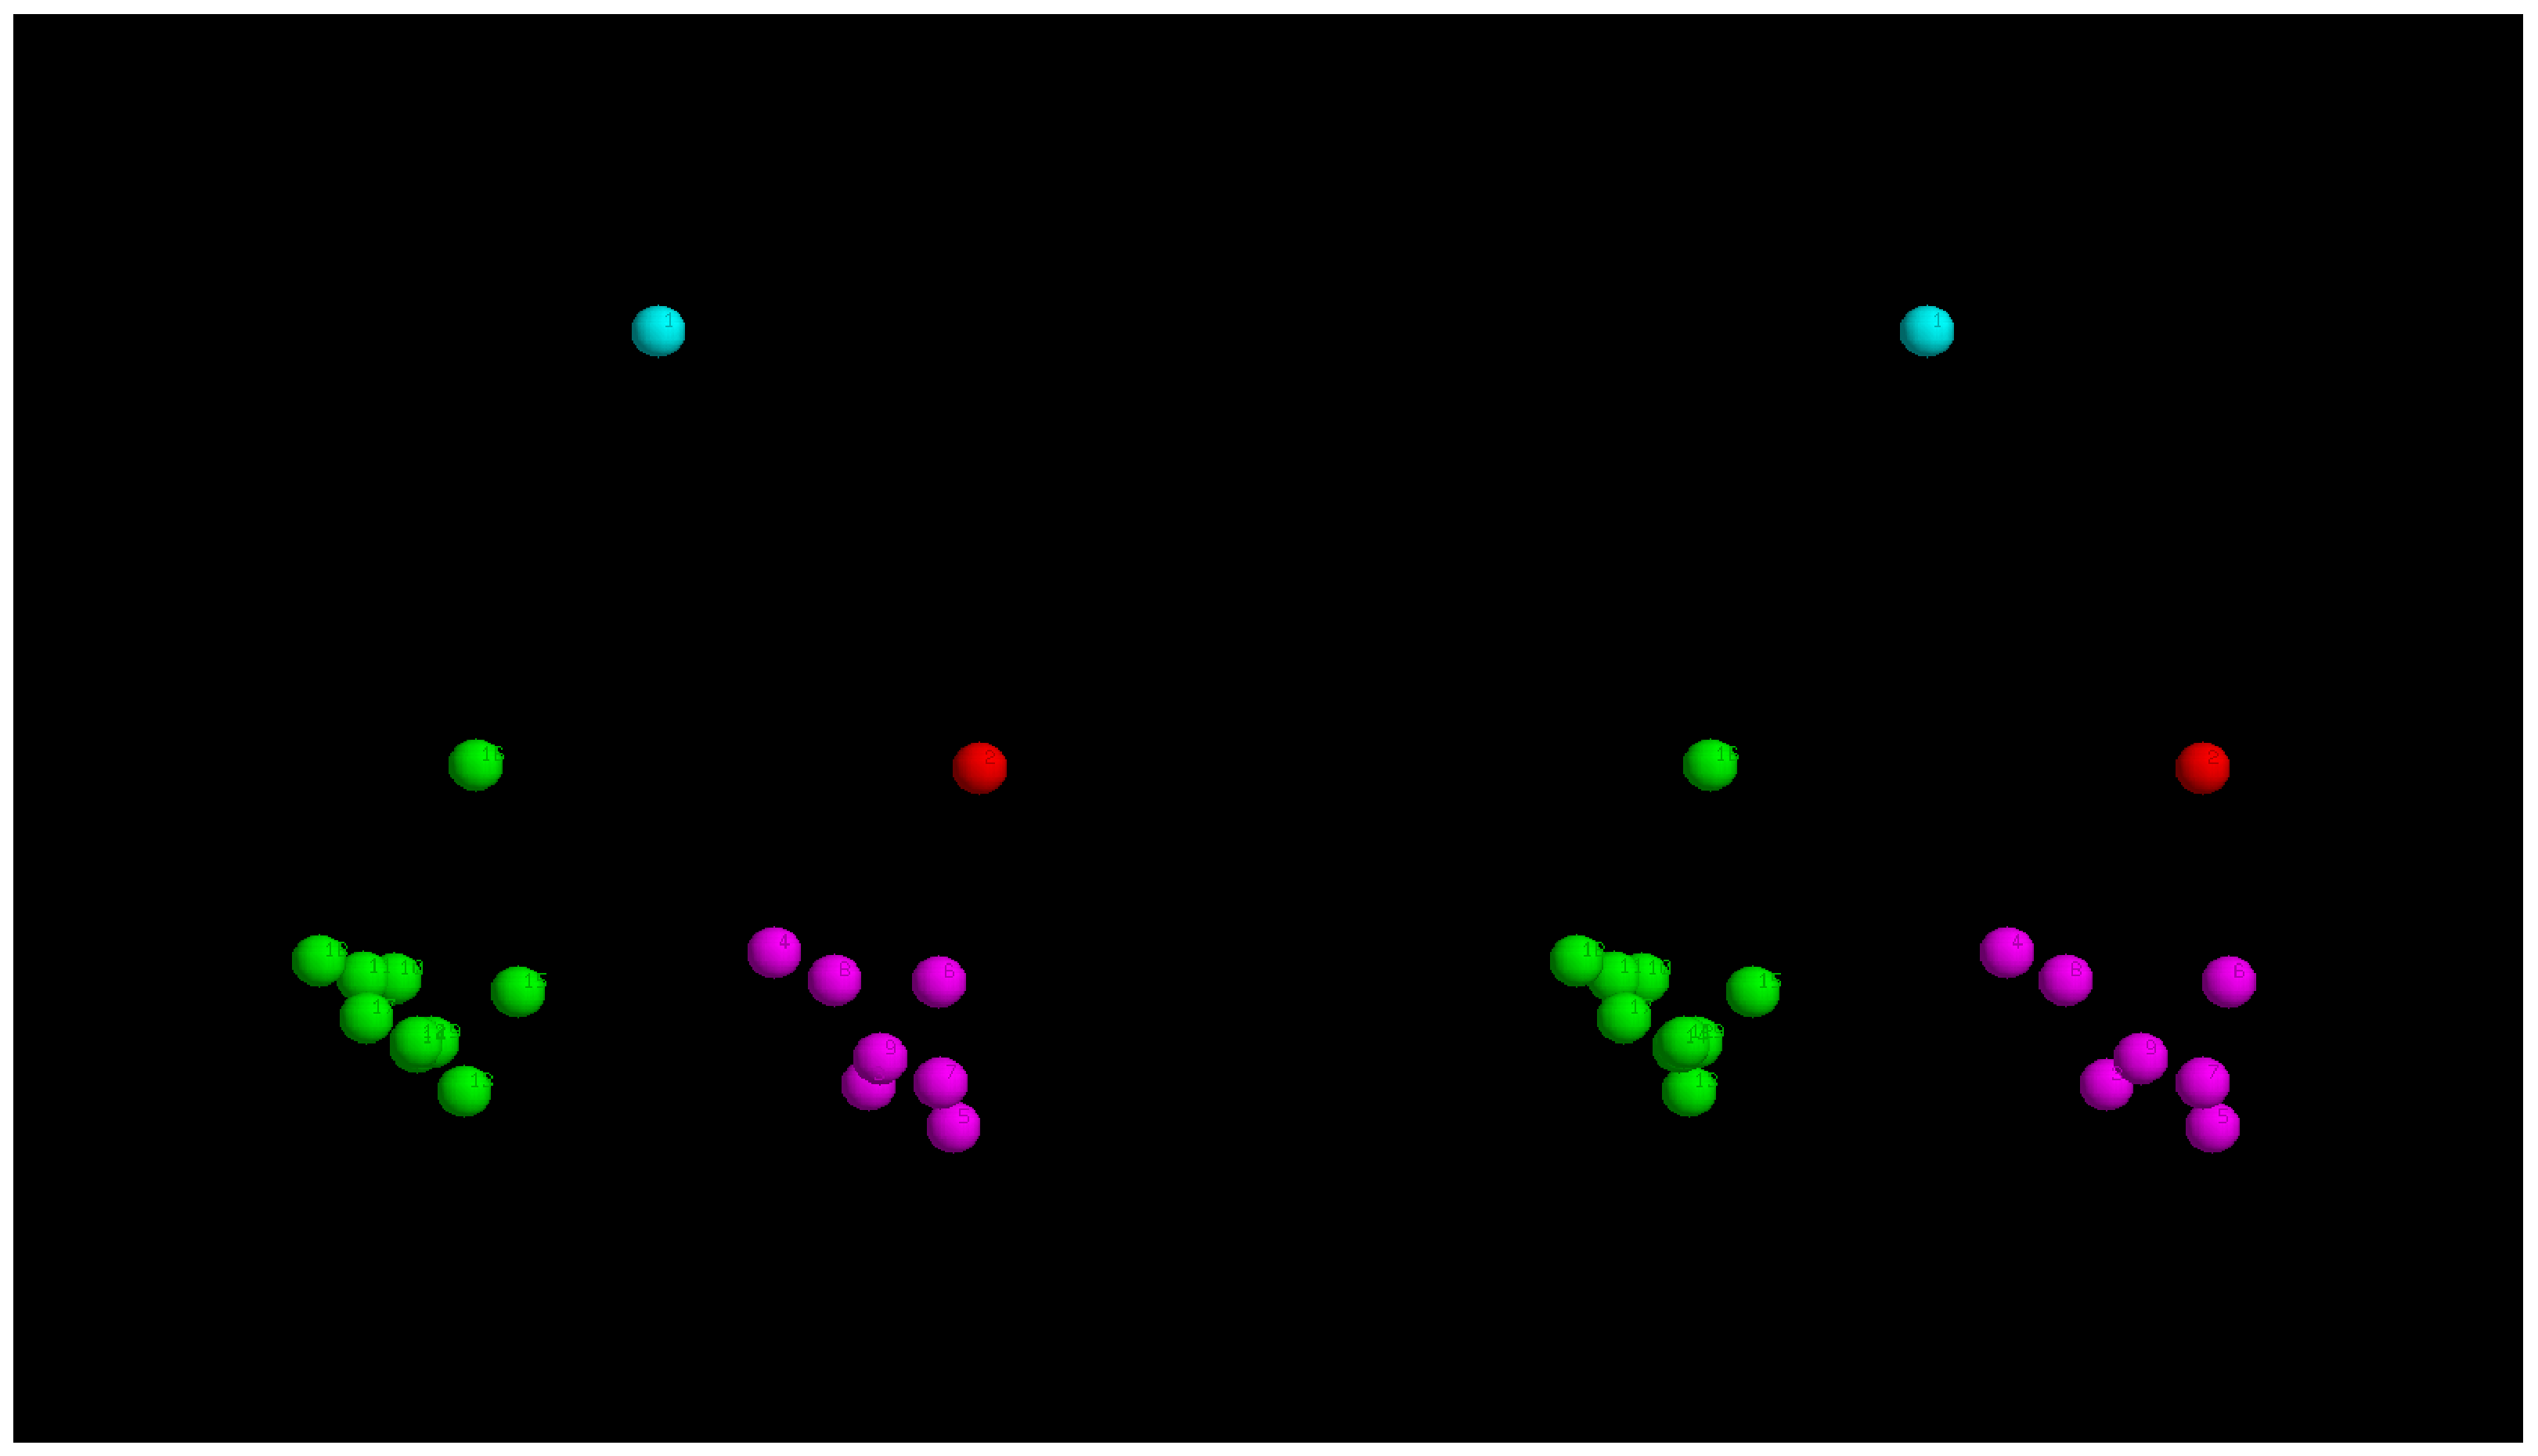
\includegraphics[width=300pt]{foldspace-space.eps}
\begin{footnotesize}
\caption{
\label{Fig:space}
{\bf Fold-space representation of all domains}.
All the viral domains considered in the paper were projected into a 3D fold-space representing
the relationship of their \SAP\ weighted RMSD values.   The domains are coloured as:
foamyN = cyan, foamyC = red, orthoN = green and ortho C = magenta.
}
\end{footnotesize}
\end{figure}

\section{Conclusions}

\subsection{Structure comparison}

\subsubsection{Pairwise significance}

The comparison of small domains that are largely composed of \A-helices presents a challenging problem in how
to interpret the significance of the RMSD values.  As the individual helical secondary structure elements
(SSEs) constitute a sizeable fraction of the domain, it takes only the chance alignment of a few helices
to result in a low RMSD over a large proportion of the structure, giving an apparently meaingful result.

The use of the customised decoy-model sets, as illustrated here, attempts to avoid this problem by recreating
a large number of possible folds that were generated using the same (reconnected) SSEs. Moreover, to avoid any
chance recreation of native fragments, each comparison always involved the comparison of a native (forward)
chain direction with a reversed chain.  Using these models, a background distribution of decoy/decoy comparisons
allowed us to calculate Z-scores for each native/native comparison between the different Gag proteins. This has
the advantage that every comparison in the background distribution involved two models with the same length,
residue packing density and secondary composition as the native pair.  These values indicated a clearly
significant relationship between the foamy and ortho CA structures.

\subsubsection{Direct or transposed domain order?}

Although the decoy model alignment strategy did confirm the relationship between the foamy and ortho CA
structures, the Z-scores did not point to a clear resolution of whether the domains should have a direct
correspondence (NN and CC match) or a transposed relationship (NC and CN) as significant individual matches
were found across all pairings. Testing for a bias towards more significant like-domain pairings (NN, CC)
in the list of similarities ranked by Z-score confirmed the visual bias towards a natural correspondence
but only at a marginal level of significance (around 0.05). By contrast, the application of a T-test on the
combined raw comparison data returned a very clear distinction between the direct and the transposed
relationships, clearly favouring the more natural forward order.

However, although the ‘astronomic’ probabilities calculated by the T-test seem very convincing, they
must be viewed in the light of the much lower probabilities calculated from the asymmetry statistics.
Both calculations involve assumptions and are limited by the small number of known structures so neither
can be taken as definitive. Nevertheless it would seem likely that the “true” level of significance may
lie somewhere between the two results and as both of these objective assessments point in the direction
of the NN and CC domain order, there is no reason to adopt the more unexpected transposed domain order.


\subsection{Evolutionary implications}

On the basis of these structural comparisons, and a variety of recently described functional assays \cite{BallNJet16}, 
we can conclude that the central region of the spumavirus gag gene encodes a polypeptide sequence related to that of 
the corresponding region of orthoretroviral, CA. It therefore seems reasonable to suppose that the last 
common ancestor of orthoretroviruses and spumaviruses possessed such a sequence. Moreover this region appears 
to be made up from two related all helical subdomains suggesting a gene duplication event in a common precursor. 

In our initial search employing foamy virus CA using the DALI program, we made the observation that the strongest
similarity of the foamy virus CA domains was actually with a cellular protein, Arc (Activity-Regulated
Cytoskeleton-associated protein).  Arc is required for neural synaptic growth and activity
\cite{ChowdhurySet06,ParkSet08,ShepherdJDet06,WaungMWet08} and mis-regulation and/or deletion contributes
to diseases of cognition \cite{NiereFet12,ParkSet08,WaungMWet08}.  Arc has widespread and clear sequence
homologues as far back as insects and probably deeper, giving it a very ancient origin somewhere close to the
metazoan root \cite{CampillosMet06,VolffJN09} and based on sequence homology Arc is considered to be a relic
of an ancient Ty3/Gypsy retrotransposon \cite{ZhangWet15}, preserved as a ’living fossil’ in metazoan genomes.
Given the structural relatedness of foamy virus CA and Arc, this might suggest an equally ancient origin for
foamy virus CA. As it is believed that the Ty3/Gypsy family of retrotransposons gave rise to retroviruses
\cite{LlorensCet08}, it will therefore be of considerable interest to determine whether the Gag of Ty elements
also comprise CA proteins with a two-domain structure.

It is also noteworthy that Ty3 Gag is significantly smaller than that of the foamy and orthoretroviruses and
although it contains CA related sequences there is no equivalent of either orthoretroviral MA or PFV Gag-NtD,
regions of Gag necessary for membrane targeting, budding and extracellular release of virions. Therefore, given
the very different structures of MA \cite{HillCPet96,PrchalJet12,RaoZet95,RiffelNet02} and Gag-NtD
\cite{GoldstoneDCet13}, this raises the possibility that the MA and Gag-NtD domains of the orthoretroviruses 
and foamy viruses were co-opted by independent events that has resulted in the viruses employing different 
mechanisms to facilitate budding from the cell. Notably, Gag from Gypsy, an Errantivirus capable of extracellular 
replication \cite{SongSUet94} and Arc contain additional N-terminal domains. In Gypsy-Gag this domain is distantly 
sequence-related to orthoretroviral MA \cite{CampillosMet06}. By contrast, in Arc it contains a coiled coil region
\cite{ZhangWet15} reminiscent of spumavirus Gag-NtD \cite{GoldstoneDCet13,TobalyJet01} further supporting the 
notion of a shared origin for Arc and foamy virus Gag that is distinguishable a from an alternative acquisition 
pathway giving rise to Gypsy and the orthoretroviruses.


\section{Methods}

\subsection{Structural data}

The foamy virus structures were obtained from the Protein Structure Databank
(PDB code:{\tt 5M1G}) \cite{BallNJet16}.

The ortho virus structures used, with their shorthand code in bold and PDB code in teletype, were:
\begin{itemize}
\item {\bf BLV}:  bovine leukemia virus (deltaretrovirus) {\tt 4PH1} (N-ter.dom) and {\tt 4PH2} (C-ter.dom) \cite{ObalGet15},
\item {\bf BLV6}: bovine leukemia virus (hexameric) {\tt 4PH0} (both dom.s) \cite{ObalGet15},
\item {\bf HIV1}: human immunodeficiency virus 1 (lentivirus) {\tt 1AK4} (N-ter.dom) \cite{GambleTRet96} and {\tt 1A43} (C-ter.dom) \cite{WorthylakeDKet99},
\item {\bf HIV6}: human immunodeficiency virus 1 {\tt 3H47} (both dom.s) \cite{PornillosOet09},
\item {\bf HML2}: human endogenous retrovirus type-K (betaretrovirus) {\tt } \cite{MortuzaGBet08},
\item {\bf HTLV}: human T-cell leukemia virus (deltaretrovirus) {\tt 1QRJ} (both dom.s) \cite{KhorasanizadehSet99},
\item {\bf JSRV}: jaagsiekte sheep Retrovirus (betaretrovirus) {\tt 2V4X} (N-ter.dom) \cite{MortuzaGBet09},
\item {\bf MLV}:  murine leukemia virus (gammaretrovirus) {\tt 1U7K} (N-ter.dom) \cite{MortuzaGBet04},
\item {\bf MPMV}: Mason-Pfizer monkey virus (betaretrovirus) {\tt 2KGF} (N-ter.dom) \cite{MacekPet09},
\item {\bf PSIV}: prosimian immunodefficiency virus (ancient lentivirus) {\tt 2XGV} (N-ter.dom) \cite{GoldstoneDCet10},
\item {\bf RELIK}: rabbit endogenous lentivirus type-K (ancient lentivirus) {\tt 2XGU} (N-ter.dom) \cite{GoldstoneDCet10},
\item {\bf RSV}:  Rous sarcoma virus (alpharetrovirus) {\tt 3G1I} (both dom.s) \cite{BaileyGDet09}.
\end{itemize}

\subsection{Structure comparison}

\subsubsection{\DALI}

The \DALI\ method for searching the PDB with a structural query \cite{HolmLet93a}
was accesed via the server at:
{\tt http://ekhidna.biocenter.helsinki.fi/dali\_server}.
The \DALI\ method reports the significance of each match with an estimated Z-score
which is the raw comparison score, normalised by the combined length of the proteins.
Z-scores down to a value of 2 are reported by the program.

The list of \DALI\ hits (ranked by Z-score) were assessed by how many high-scoring capsid structures had
been identified.    These true/false (T/F) hits were defined simply by protein descriptions that contained the
words "CAPSID", "GAG" or "P24".   This may have misclassified a few (low scoring) hits to the matrix protein
and missed some hits where the primary description refers to a cyclophilin structure solved in complex
with the capsid.

\DALI\ reports structural hits in both the full PDB and a reduced collection of structures that
have no pair of proteins with over 90\% sequence identity, referred to as the 90\% non-redundant or PDB-90 collection.
It was found, however, that some hits, seen in the full PDB were not found in the PDB-90, for example in \Fig{revs},
all of the top 31 hits of the N-domain against the full PDB are missing in the PDB-90 hits.
The most likely explanation is that the PDB-90 secection has not been updated at the same time
as the full collection.    For this reason, hits to both databases were monitored.

\subsubsection{\SAP}

The \SAP\ method for structure comparison \cite{TaylorWR99a} was run as a local copy which can
be accessed at: {\tt https://github.com/WillieTaylor/util}.  
As part of determining the alignment between two structures,
the \SAP\ program calculates a similarity score for each pair of matched positions which is
how similar the rest of the structure looks from the viewing-frame of the superposed residues.
This value can be used both to weight the importance of positions when calculating the
(rigid-body) RMSD superposition and to colour positions in the superposed structures.
\cite{RippmannFet91a}. (As in \Fig{top2}).

If the matched positions are ranked by this value, then RMSD values can be calculated over
increasingly larger subsets to high-light the extent of a well matched core before
the contribution of variable loops, or domain shifts, leads to higher RMSD values.
(As in \Fig{fullRMS}).

\subsection{Decoy structure construction}

\subsubsection{Reversed structure decoys}

Simple structural decoys were generated from native PDB structures by reversing the order
of the \CA\ atoms in the PDB file using the Unix command line:
\begin{verbatim}
cat native.pdb | grep ' CA ' | sort -nr -k2 > reverse.pdb
\end{verbatim}
The reversal of a protein chain does not alter the chirality of the alpha helix and
these decoys can be used directly in \SAP.   However, \DALI\ requires all main-chain atoms
and these must be regenerated for the reversed decoys.   This was done using the simple
{\tt ca2main} program which can also be found at: {\tt https://github.com/WillieTaylor/util}.

\subsubsection{Customised decoys}

Customised structural decoys were generated for each comparison using each of the
pair of structures being compared to create two pools of decoys then comparing all
decoys in the first pool against all decoys from the second but with their chain
reversed as described in the previous section.

The decoys were created as described in Ref.\cite{TaylorWR06a}: starting by cyclising the
chain then introducing new termini in each surface loop to create cyclic permutations.
In addition, when three loop regions lie in close proximity, their ends are also
reconnected in such a way that if a chain, comprising four segments ($1\ldots4$) runs 
from amino (N) to carboxy (C) termini through three adjacent loop regions {\tt a-b},
{\tt c-d} and {\tt e-f} (i.e.: N,{\tt 1,a-b,2,c-d,3,e-f,4},C) then the reconnected chain
runs: N,{\tt 1,a-d,3,e-b,2,c-f,4},C with each switch being made at the least disruptive
point between a pair of loops.   This chain switching does not create any reversed segments
which would otherwise form regions of local matching when the whole chain is reversed.

In a pair of structures, if each have four surface loops where breaks can be made, then
including the native termini, this gives five cyclic permutations and if two groups of
loops can be reconnected then a total of 15 distinct decoys can be made from each native
starting structure.   As these can be compared pairwise, a pool of 225 decoy derived
data points is generated that constitutes the random background against which the native/native
comparison can be assessed.

For example, in \Fig{sapit}, the 36 data
points marked by a solid circle come from the comparison of six cyclic permutations of a
native ortho domain compared with six permutations of a reversed foamy domain that includes
a single loop reconnection.

Every pair drawn from this pool will have the same lengths as the two native structures
as well as the same secondary structure composition, surface exposure, residue packing
density and inertial properties but each decoy will have a different chain fold.


\subsection{Statistical tests}

\subsubsection{RMSD length normalisation}

The quality of structure comparisons can be characterised by a combination of their
RMSD value and the number of matched (superposed) positions.  How to combine these values has
been the subject of much discussion over the years and central to this is the expected random
RMSD value for two proteins of a given length \cite{McLachlanAD84,CohenFEet80d,MaiorovVNet94}.   However,
when reviewed \cite{TaylorWR06a}, all these measures were approximations of a simple square-root function of
the protein length (as originally proposed by McLachlan on theoretical grounds \cite{McLachlanAD84})
but with an added term to depress the RMSD values obtained with small units or structure
that are dominated by secondary structure elements (and super-secondary structure motifs)
giving a lower than expected RMSD value.   The formula that best captures this is:
$R = \surd N (1-\exp(-N^2/s^2))$,
where,
$R$ is the expected random RMSD for $N$ matched positions and $s$ is the damping factor in the inverted
Gaussian term (equivalent to the standard deviation in the Normal distribution).

Any point that lies on this line can be considered "exactly" random
with those above it being "more" random and those below it "less" random.  This can be quantified
as a single number which is the value of a scaling factor ($a$), which when applied to the curve, makes it
pass through any given point.   If a comparison has an RMSD of $R$ over $N$ positions, then
$R = a\surd N (1-\exp(-N^2/s^2))$ and when
\begin{equation}
\label{Eqn:fit}
a = R/(\surd N (1-\exp(-N^2/s^2))), 
\end{equation}

the line will pass through the data point.  This reduces the pair of values ($R,N$) to a
single value $a$ that is a simpler quantity for statistical analysis.

The best value for $s$ is slightly dependent on the nature of the proteins being compared.
For artifical (random-walk)  models with no secondary structure, no modification will be needed but the
proteins considered here have segments of packed alpha helices that can be locally similar
over two to three helices.   To correct for this, a value of $s=30$ was used (or $1/s^2 = 0.11$)
which is higher than the value of $1/s^2 = 0.03$ used previously.
That this is a reasonable fit to the data can be seen in the way the dashed blue lines
in \Fig{sapit} track the upper and lower boundary of the decoy comparison results.

When $a=1$, the point lies on the random line and when $a=0$, the RMSD is zero, so values of
$a$ that approach this lower bound will be of interest when evaluating similarity.

\subsubsection{Frequency plots}

The $a$-values obtained using \Eqn{fit} were plotted as frequency histograms using using
only data points that had a length of $N\pm 10$, where $N$ is the maximum number of matched
positions in the comparison of the two native structures.   
Previously, a cumulative plot of RMSD was used to select an optimal value for
$N$ (giving the minimum $a$-value).   This can be important if the full set of matched
positions is dominated by a high deviations from variable loop regions.   However, in the
current application, the small length of the foamy virus loops meant that this was not
an important aspect and the full number of matched positions was taken.   Otherwise, the
same correction would have to be applied to all decoy comparisons to maintain a fair
comparison.  (See \Fig{sapit}, where the black dot marks the minimum $a$-value length).

The mean and standard deviation of the $a$-values in the $N\pm10$ region were calculated
and the corresponding Normal distribution used to calculate Z-scores for the associated
native comparison. (See \Fig{normHIV}, for an example).

\subsubsection{T-tests}

Data from separate native/native comparisons, with their customised decoy data, were combined
giving not only a much larger background population of decoy derived scores but also a small
population of native comparison scores that can be tested to calculate the probability that
they were drawn from the same population as the decoy data.  To do this, a T-test was used which
takes the size, mean, and standard deviation of each distribution and calculates a probability.
The implementaion of this test was taken from the Numerical Reicpies collection \cite{PressWHet86}
which implements one of two variants of the test depending on whether the distributions
have statistically distinct standard deviations. (Routines {\tt ttest()} and {\tt tutest()}).
The choice of routine is based on a preapplication of an F-test on the standard-deviations.
(Using the routine {\tt ftest()}).

The values quoted in the Results section are for a two-tailed T-test, however, as it is expected
that the native comparisons should always be more similar than comparisons between random models,
then a one-tailed T-test would be valid, which gives half the probability.   As the values
in the Tables are so significant and only the relative relationships are of interest,
then the choice is unimportant.

\subsection{Fold-space clustering}

The results of the pairwise similarity within a set of structures can be visualised by treating the
RMSD values as Euclidean distances\footnote{In theory, pairwise RMSD values are guaranteed to constitute
a consistent Euclidean metric, but only in N-1 dimensions (where N is the number of structures compared).
} and reducing their dimensionality to sufficiently few dimensions to be visualised: usually 2D or,
better 3D, to visualise the space with less distortion.
Rather than use a simple multi-dimensional scaling (MDS) method (\cite{BrownNPet96}), the more complicated
method of multi-dimensional projection was used (\cite{AszodiAet97a}, see \cite{TaylorWRet01b} for a
simpler exposition).

This method reduces the dimensionality of the projection in gradual stages
with each step employing triangle-inequality balancing and hyper-dimensional real-space refinement.
In the real-space refinement stages, a weight can be applied to pairwise distances. (This cannot be
done in direct MDS projection, which can only assign a mass to each point).
Weights were assigned to distances as a function of their inverse RMSD, up to a maximum value of 1.

The method is robust and
has been widely applied to rough models (\cite{TaylorWRet09a}) and predicted inter-residue distances that
constitute highly non-metric data sets (\cite{AszodiAet94a}).



%% The Appendices part is started with the command \appendix;
%% appendix sections are then done as normal sections
%% \appendix

%% \section{}
%% \label{}

%% References
%%
%% Following citation commands can be used in the body text:
%% Usage of \cite is as follows:
%%   \cite{key}          ==>>  [#]
%%   \cite[chap. 2]{key} ==>>  [#, chap. 2]
%%   \citet{key}         ==>>  Author [#]

%% References with bibTeX database:

\bibliographystyle{model1-num-names}
\bibliography{newrefs,pdbrefs,jonrefs}

%% Authors are advised to submit their bibtex database files. They are
%% requested to list a bibtex style file in the manuscript if they do
%% not want to use model1-num-names.bst.

%% References without bibTeX database:

% \begin{thebibliography}{00}

%% \bibitem must have the following form:
%%   \bibitem{key}...
%%

% \bibitem{}

% \end{thebibliography}

\paragraph{Acknowledgements:}
The work was supported by the Francis Crick Institute under awards: FC001179 (WRT), FC001162 (JPS) and FC001178 (IAT).
The Crick receives its core funding from Cancer Research UK, the UK Medical Research Council, and the Wellcome Trust.


\end{document}

%%
%% End of file `elsarticle-template-1-num.tex'.
